\chapter{Methods common to all chapters}



\todo{We should move some of the introduction here as methods esp the bit about gene-level tests}
This thesis will address how network studies inform two of the approaches to the understanding of differences in intelligence and their association with models of the synapse.



\todo{perhaps change this to cohort generation and network graph and add the network level statistics from the next chapter to this or split into two chapters the network grapha nd network level statistics and cohort generation and gene level results}
\todo{you could also add the Hill revisited GSA and the gsa from the MAGMA site gene set synaptic into this section}


``Pathway" based approaches study for genetic variants the genes that are associated with cognition in model organisms \cite{deary2009genetic} (the ``genes to cognition" project being an example). These have therefore primarily addressed the consequence of molecular perturbation primarily of synaptic proteins. 

The other, population genomic approach examines large numbers of individuals in Genome Wide Association Studies and determines how the specific genetic differences they have influence differences in educational attainment and intelligence. These require large studies to develop sufficient power as the individual effect of these genetic differences is small \cite{plomin2015genetics}. In the course of completing this thesis the number of individuals included in the samples  available to me has increased dramatically (see fig) \todo{add figure}. Before seeing how these studies are correlated with the structure of the synaptic network we must first generate the network. 


\section{Network Graph}
\label{sec:network graph generation}

An undirected, unweighted interaction network graph was generated to represent the protein-protein interactions of the post synaptic density (PSD) and its essential interaction partners. This graph allows use to see in the interaction logic of the post synaptic density and closely associated proteins. The nodes (vertices) in the graph are the cognate genes for proteins found in the post synaptic density or in proteomic analysis of the density. An edge occurs between genes if there is directed experimental evidence that their protein products interact. 




The generation of the network from the literature was carried out by OS,CMcL,JDA,IS,KH etc\todo{get list from JDA} and I was not involved in this process.

39 proteomic studies conducted between 2000-2017 of the human and mouse synapses were curated into a list of 6500 potential synaptic genes (all mapped to human IDs). \cite{heil2018systems}  Of these studies, 22 examined the post synaptic density (PSD), an electron dense structure beneath the post synaptic membrane \cite{PALAY1956}  consisting of complexes of neurotransmitter receptors and their supporting proteins. \cite{kennedy2000signal}  Affinity purification against common PSD proteins improves their identification. \cite{ewing2007large}  The human proteins and human orthologues of mouse proteins found in these studies were used as a ‘parts list’ for the PSD and associated proteins expressed in the post synaptic area. We call this the post-synaptic proteome (PSP).

  A bi-map was created to translate between protein identifications, such as Uniprot\cite{uniprot2017uniprot}, and the Entrez ID of the genes that encoded them. Entrez IDs were used as the identifier for all subsequent data tables and analyses. Protein-protein interactions were obtained from the mining and harmonisation of data from the Database of Interacting Proteins (DIP), \cite{xenarios2002dip}  IntAct database, \cite{orchard2014mintact}  and BioGRID. \cite{chatr2017biogrid}  Only human interaction data was used. Protein-protein interactions were excluded if there was not direct experimental evidence of interaction documented  Proteomics Standard Initiative - Molecular Interaction ontology terms (PSI-MI)\todo{check ref with Douglas ? use PSIMI 3.0 but uncited and only available as web resource} in the databases. PSI-MI is a structured ontology used to describe protein protein interactions.\cite{isserlin2011biomolecular} PPIs based on 'genetic interactions', 'genetic interference', and 'co-localisation' were excluded.

 The network graph used for subsequent analysis in this thesis is the largest connected component of the complete network induced by the genes derived from PSP parts list on network interactions filtered for high quality interaction (one study has been removed because of \todo{ADD}. The complete network graph contains 3473 vertices and 30499 edges. 
 
The largest connected component of the resulting graph was used for community detection and in calculating network statistics (3457 nodes, 30498 edges). The details of the small number of excluded vertices not part of the largest connected component are in section~\ref{sec: PSP graph connected component and missing} below.

The methods for generation of the graph are described in detail in \cite{heil2018systems}. The vertex and edge lists are available in Supplementary material X. 

The network was stored as a graph modelling language (GML) file and transformed to other formats such as ncol or gexf from this original file.\cite{himsolt1997gml}  A master copy of the original file supplied to me was stored on the University of Edinburgh informatics server. The original gml file was generated by CMcL and is included in the supplementary material.

\subsection{Connected component}
\label{sec: PSP graph connected component and missing}
In addition to the giant connected component 15 smaller components were found within the PSP graph all single isolated components other than one component of size 2. The cognate proteins of these genes appear in the ``parts list" derived from proteomic studies but lack experimental evidence of direct interaction with the protein products of the genes in the giant component of the PSP. Community detection algorithms and most vertex statistics are not valid for unconnected components and these vertices were excluded. The composition of the excluded components was analysed  to assess whether they contained elements that might bias the subsequent analyses. \todo{do GSA for these component} For further discussion of connected component see section~\ref{sec:connected component and degree}.

\subsection{Gene ontology analysis}
\label{sec: gene ontology analysis}
A gene ontology provides a controlled, maintained vocabulary to described sets of genes according to their Biological Function, Cellular Component and Molecular Function and is commonly used in high throughput genetics to provide information on the function of a set of genes. \cite{ashburner2000gene}
Gene ontology over-representation analysis was carried out using PANTHER version 13.1.\cite{mi2013large}



\subsubsection{Analysis of Genes not in largest connected component}
\label{sec:analysis of genes not in largest component}
16 genes were not in the giant connected component.The genes are listed in table~\ref{table:notinLCC}. The final column indicates the number of genes in the component. The only two gene component was composed of oligodendrocyte myelin glyocprotein (OMG) and reticulon 4 receptor (RTN4R). 

Gene ontology analysis was carried out to test for differential representation of Gene Ontology terms in the 16 genes not in the giant connected component. PANTHER 13.1.\cite{mi2013large} was used to carry out testing for each of the three Gene Ontology clades (cellular component, biological process or molecular function) using Fishers exact test. The Benjamini-Hochberg procedure \cite{benjamini1995controlling} was used to calculate the False Discovery Rate (FDR) to account for multiple comparisons.

No statistically significant enrichment of ontology terms was found after correcting for multiple comparisons. 

All but 0.46\% (S= 0.995) of the genes in the parts list are part of the largest component. This is comparable to the figure for S of 0.996 for undirected metabolic networks in \cite{newman2018networks} p 305 but high compared to the n=2115 Protein interaction with S=0.689 in the same reference). \todo{So what}\footnote{Code to generate the table is found at \url{'~/RProjects/analyse_DICE_data/R/LCC.R'}}

%%% GENES EXCLUDED AS NOT IN LCC %%%

% latex table generated in R 3.6.2 by xtable 1.8-4 package
% Tue Dec 31 09:25:51 2019
\begin{table}[ht]
\centering
\begin{tabular}{cllc}
\toprule
 
Entrez Gene ID & Gene Symbol & Gene Name & n in component \\ 
\midrule
 4974 & OMG & oligodendrocyte myelin glycoprotein & 2 \\ 
  65078 & RTN4R & reticulon 4 receptor & 2 \\ 
 98 & ACYP2 & acylphosphatase 2 & 1 \\ 
  166785 & MMAA & metabolism of cobalamin associated A & 1 \\ 
  549 & AUH & AU RNA binding methylglutaconyl-CoA hydratase & 1 \\ 
  55847 & CISD1 & CDGSH iron sulfur domain 1 & 1 \\ 
  23305 & ACSL6 & acyl-CoA synthetase long chain family member 6 & 1 \\ 
  26027 & ACOT11 & acyl-CoA thioesterase 11 & 1 \\ 
  7915 & ALDH5A1 & aldehyde dehydrogenase 5 family member A1 & 1 \\ 
  4685 & NCAM2 & neural cell adhesion molecule 2 & 1 \\ 
 
  5649 & RELN & reelin & 1 \\ 
  2741 & GLRA1 & glycine receptor alpha 1 & 1 \\ 
  152404 & IGSF11 & immunoglobulin superfamily member 11 & 1 \\ 
 
  27000 & DNAJC2 & DnaJ heat shock protein family (Hsp40) member C2 & 1 \\ 
  2686 & GGT7 & gamma-glutamyltransferase 7 & 1 \\ 
  55262 & MAP11 & microtubule associated protein 11 & 1 \\ 
   \bottomrule
\end{tabular}
\caption{Genes with cognate proteins in the PSP as defined by their presence in proteomic studies but that are not part of the giant connected component. These are elements therefore that lack direct experimental evidence of interaction with the giant connected component. } 
\label{table:notinLCC}
\end{table}
%%%


\subsection{Gtex profile of PSP genes}
\label{gtex profile of PSP genes}
\subsubsection{Introduction to gtex}
The gene tissue expression project (GTEx) is a repository of gene expression in over 1000 individuals from 54 tissue areas. I have used this to determine if the PSP genes are predominantly expressed in the brain, if there are significant regional differences in expression that might affect the analysis and that the expression of PSP genes is as expected significantly greater than of those not in the PSP, which will of course include a number of genes significantly involed in processes in the brain. 

\subsubsection{Methods}
The data used for the analyses of post synaptic proteome gene expression described in this manuscript were obtained from: the GTEx Portal on 07/03/2020. Median gene expression counts normalised by Transcripts Per Million (TPM)  were downloaded from the GTEx Portal website \footnote{ \url{https://storage.googleapis.com/gtex_analysis_v8/rna_seq_data/GTEx_Analysis_2017-06-05_v8_RNASeQCv1.1.9_gene_median_tpm.gct.gz}}.Two indexes were provided for data ensembl id and gene symbol. The toppgene annotation service was used to provide entrez ids from gene symbol to allow the results to be combined with the synaptic network and cohort study results \todo{may not have mentioned the cohorts yet}.\cite{gtex2015genotype},\cite{conesa2016survey}
\subsubsection{Correlation of genes across brain areas}
% latex table generated in R 3.6.3 by xtable 1.8-4 package
% Sat Mar  7 15:12:52 2020
There is strong correlation correlation between gene expression counts in all brain regions see table~\ref{Correlation between brain regions in expression of all genes in Gtex}. Therefore for simplicity median gene expression for the cortex was used in further analyses. 

\begin{table}[ht]
\centering
\begin{adjustbox}{width=\textwidth}
\begin{tabular}{rrrrrrrrrrrrrr}
  \hline
 & Amy & AntCing & Caudate & Cerebellar H & Cerebellum & Cortex & Frontal & Hippocampus & Hypothalamus & NA & Putamen & Spinal & S. nigra \\ 
  \hline
Amygdala & 1.000 & 0.999 & 0.997 & 0.996 & 0.995 & 0.999 & 0.995 & 0.999 & 0.999 & 0.999 & 0.996 & 0.984 & 0.993 \\ 
  Anterior cingulate cortex(BA24) & 0.999 & 1.000 & 0.999 & 0.996 & 0.992 & 0.999 & 0.998 & 0.999 & 0.999 & 1.000 & 0.999 & 0.981 & 0.996 \\ 
  Caudate (basal ganglia) & 0.997 & 0.999 & 1.000 & 0.995 & 0.988 & 0.997 & 0.999 & 0.998 & 0.998 & 0.999 & 1.000 & 0.981 & 0.998 \\ 
  Cerebellar Hemisphere & 0.996 & 0.996 & 0.995 & 1.000 & 0.996 & 0.997 & 0.995 & 0.995 & 0.996 & 0.996 & 0.994 & 0.978 & 0.991 \\ 
  Cerebellum & 0.995 & 0.992 & 0.988 & 0.996 & 1.000 & 0.996 & 0.986 & 0.992 & 0.992 & 0.992 & 0.986 & 0.975 & 0.981 \\ 
  Cortex & 0.999 & 0.999 & 0.997 & 0.997 & 0.996 & 1.000 & 0.996 & 0.999 & 0.999 & 0.999 & 0.996 & 0.981 & 0.992 \\ 
  Frontal Cortex(BA9) & 0.995 & 0.998 & 0.999 & 0.995 & 0.986 & 0.996 & 1.000 & 0.997 & 0.997 & 0.998 & 0.999 & 0.978 & 0.997 \\ 
  Hippocampus & 0.999 & 0.999 & 0.998 & 0.995 & 0.992 & 0.999 & 0.997 & 1.000 & 1.000 & 0.999 & 0.998 & 0.985 & 0.996 \\ 
  Hypothalamus & 0.999 & 0.999 & 0.998 & 0.996 & 0.992 & 0.999 & 0.997 & 1.000 & 1.000 & 0.999 & 0.998 & 0.985 & 0.996 \\ 
  Nucleus accumbens (basal ganglia) & 0.999 & 1.000 & 0.999 & 0.996 & 0.992 & 0.999 & 0.998 & 0.999 & 0.999 & 1.000 & 0.999 & 0.982 & 0.996 \\ 
  Putamen(basalganglia) & 0.996 & 0.999 & 1.000 & 0.994 & 0.986 & 0.996 & 0.999 & 0.998 & 0.998 & 0.999 & 1.000 & 0.981 & 0.999 \\ 
  Spinal cord(cervicalc1) & 0.984 & 0.981 & 0.981 & 0.978 & 0.975 & 0.981 & 0.978 & 0.985 & 0.985 & 0.982 & 0.981 & 1.000 & 0.984 \\ 
  Substantia nigra & 0.993 & 0.996 & 0.998 & 0.991 & 0.981 & 0.992 & 0.997 & 0.996 & 0.996 & 0.996 & 0.999 & 0.984 & 1.000 \\ 
   \hline
\end{tabular}
\end{adjustbox}
\caption{Correlation between brain regions in expression of all genes in Gtex}
\label{Correlation between brain regions in expression of all genes in Gtex}
\end{table}

%%

\subsection{Comparison of expression in PSP and rest of genome}
Only 19 PSP genes have not recorded expression in the brain tissues of Gtex. 20998 genes of 46058 in the non synaptic have no expression. These however contain many non standard gene elements such as micro RNAs and other RNA components. A subset of genes was generated using as a filter the genes in the PSP and all genes that appear in all studies \todo{lookup and subset with expressed in study} \textcolor{red}{may want to change this to any study and will need to change graph again}. 1699 of 19244 non PSP genes had 0 count in brain cortex.



Median expression in PSP brain cortex was 21.85 and mean 100.07. THe median in non PSP genes was 3.61 and mean 11.82 (see table~\ref{tab:Summary statistics for gene expression for PSP and non PSP genes}

Mean expression in PSP genes brain cortex is higher than in non PSP. The data appear right skewed and do not appear normally distributed. T test 	Welch Two Sample t-test


t = 3.3731, df = 3391.5. 95 percent confidence interval of difference in mean :36.96 -139.56, sample estimates:mean of PSP 100.07 mean of non PSP  11.82, p-value = 0.0007517

A non parametric test 

	Wilcoxon rank sum test with continuity correction W = 51340370, p-value $< 2.2 \times 10^{-16}$


I also log 10 transformed the expression values for brain cortex and performed a t test to get an estimate of the difference in means. As there were a large number of values at 0 (which would have infinite log) is set these values log10 result to 0.

	Welch Two Sample t-test

t = 60.809, df = 5310.4, 
alternative hypothesis: true difference in means is not equal to 0
95 percent confidence interval: 0.826 - 0.881
sample estimates:mean of PSP 1.288  mean of non PSP 0.434 , p-value $< 2.2 \times 10^{-16}$. 

The distribution of log transformed median expression for cerebral cortex for PSP genes and non PSP genes included in the cohorts are shown in table~\ref{fig:all_gtex_panels}.\todo{ensure GTEx is correct ie check case throughout} \todo{Gene expression levels with centrality measures and across communities}
 
 \textcolor{red}{want to do expression psp compared with average expression in other tissues per Sniekers}

 % latex table generated in R 3.6.3 by xtable 1.8-4 package
% Sat Mar  7 17:12:57 2020
\begin{table}[ht]
\centering
\begin{tabular}{lrrrrrrr}
  \hline
group & n & Min. & 1st Qu. & Median & Mean & 3rd Qu. & Max. \\ 
  \hline
PSP & 3392 & 0 & 8.43 & 21.85 & 100.07 & 55.87 & 62949.60 \\ 
  non PSP genes & 138980 & 0 & 0.38 & 3.61 & 11.82 & 12.10 & 1288.95 \\ 
   \hline
\end{tabular}
\caption{Summary statistics for gene expression for PSP and non PSP genes calculated from GTEx project data. Expression is median normalised by TPM.}
\label{tab:Summary statistics for gene expression for PSP and non PSP genes}
\end{table}


    See figure~\ref{fig:all_gtex_panels} for a graphical comparison of expression of PSP and non PSP genes in the cortex. \footnote{code \url{source('~/RProjects/gtex/R/graph_gtex/histogram_boxplot.R')} } \footnote{code using only genes in study and removing synaptic and rest of genome duplicates \url{source('~/RProjects/gtex/R/graph_gtex/graphs_study_genes.R')} }. Table~\ref{tab:Summary statistics for gene expression for PSP and non PSP genes} shows gene expression for PSPS and non PSP genes \footnote{\url{source('~/RProjects/gtex/R/graph_gtex/graphs_study_genes.R')}}
    
    
    
\begin{figure}
    \centering
    \begin{subfigure}[t]{0.45\textwidth}
        \centering
        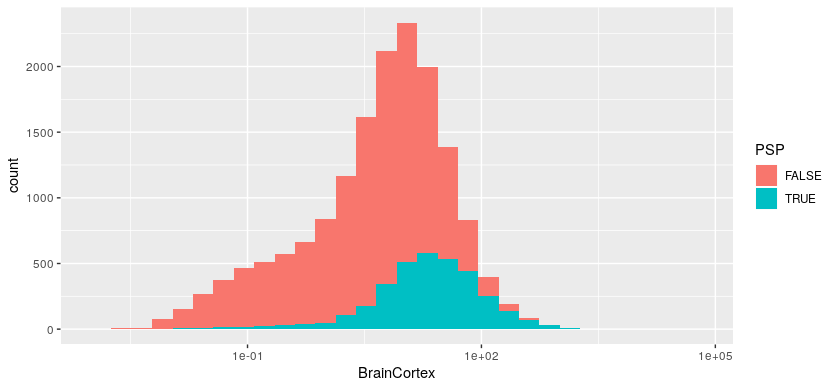
\includegraphics[width=\linewidth]{images/Rplot_corrected_gtex_histogram_log.png} 
        \caption{Histogram of expression PSP and non PSP. Log10 scale} \label{fig:gtex_histogram_log}
    \end{subfigure}
    \hfill
    \begin{subfigure}[t]{0.45\textwidth}
        \centering
        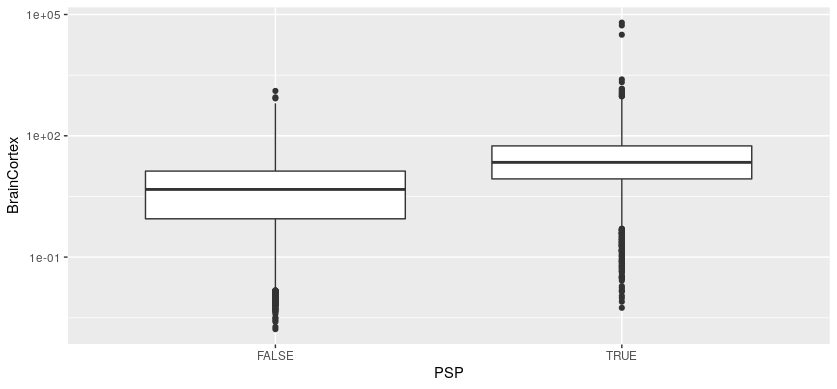
\includegraphics[width=\linewidth]{images/Rplot_corrected_gtex_boxplot_log10.png} 
        \caption{Gtex expression boxplot PSP against not PSP. Log10 scale} \label{fig:gtex_log_boxplot}
    \end{subfigure}
    \caption{Plots of gtex expression \textcolor{red}{may want to do this in subfigure packages rather than subcaption to line up edges and tidy up images in ggplot}}
    \label{fig:all_gtex_panels}
\end{figure}

\section{Genome Wide Association Studies}

To carry out inference about the association between network properties and structures and population genetic variation associated with intelligence we will need to calculate a significant test for each vertex gene. These will be calculated using MAGMA in four samples, two of intelligence and two of educational attainment.\cite{de2015magma}


\subsection{Cohorts}
\label{sec:cohorts from paper section}
%\textcolor{red}{from paper section}
Later in this thesis to investigate the efficacy of community detection in the analysis of GWA studies of cognitive ability and educational attainment I will use a discovery and replication cohort design. For consistency therefore I will refer throughout the text to the GWA study of genetic variants associated with intelligence in UK Biobank\cite{bycroft2018uk} as Intelligence\textsubscript{Discovery}  and the Phase II Educational attainment GWA study conducted using UK Biobank as Education\textsubscript{Discovery}.

We refer to the meta-analytic GWAS of intelligence carried out by Sniekers et al from the Complex Trait Genetics (CTG) lab as Intelligence\textsubscript{Replication}. \cite{sniekers2017genome}   The meta-analysis of GWA studies of educational attainment excluding UK Biobank and 23 and me by Okbay et al is referred to as Education Replication or EA2. \cite{okbay2016genome}. Details of these samples are found in the following section~\ref{sec:samples from paper section}. 

Two further samples became available after the completion of the primary analysis consisting of the largest intelligence and education cohorts to date \cite{savage2018genome}, \todo{add EA3}

\subsection{Samples}
\label{sec:samples from paper section}

Intelligence and education were the two cognitive phenotypes used to examine the effect of network structure and network communities \todo{rephrase this section}. The discovery sample for intelligence was formed using the ‘fluid’ cognitive test from UK Biobank; we shall refer to it as verbal-numerical reasoning (VNR). The VNR test contains 13 multiple choice items, six of which are verbal with the remaining seven being numerical in nature. Each individual’s VNR score was the sum of correct responses attained within a two-minute time period. This test has a large genetic correlation with intelligence scores derived from psycho-metrically validated cognitive tests. A total of 120 934 participants (mean $\chi^2$=1.52) were available for analysis who did not contribute data to the Sniekers et al data set. A full description of how data from these participants was analysed can be found in Hill et al. \cite{hill2019combined} 
UK Biobank was also used as the discovery sample for education. Summary statistics were taken from Hill et al on 273 274 participants (mean  $\chi^2$= 1.67). \cite{hill2019combined}  Education was defined as a binary choice of whether or not the individual had a University/College degree. A full description of how these data were analysed can be found in Hill et al. \cite{hill2019combined}  
To attempt to replicate any findings of enrichment for post synaptic communities, an intelligence replication dataset was formed using summary statistics obtained from the Sneikers et al. GWAS meta-analysis of intelligence (n = 78 308, mean $\chi^2$= 1.30).  \cite{sniekers2017genome}  An education replication data set was formed using summary data set from the GWAS meta-analysis by Okbay et al (n = 217 569, mean $\chi^2$= 1.43) with UK Biobank participants excluded. \cite{okbay2016genome}  (See supplemental tables 1a and 1b.)
\textcolor{red}{end from paper section}

 
\subsection{MAGMA Gene level statistics validation from other studies}

In order to ensure the accuracy of the gene level significance statistic we compared the gene level scores obtained using MAGMA to those reported in available studies.\cite{de2015magma} There were no published papers available containing a MAGMA gene-level analysis for the UK Biobank Intelligence cohort (Intelligence\textsubscript{Discovery} nor the UK Biobank Educational attainment cohort. The EA2 \cite{okbay2016genome} educational attainment paper did not report MAGMA gene scores, and in addition the Education\textsubscript{Replication} sample differs from the EA2 cohort by not including UK Biobank Educational attainment data. The only published paper reporting MAGMA gene scores from our discovery and replication cohorts of was, therefore, the Intelligence\textsubscript{Discovery} sample \cite{sniekers2017genome} (supplementary table 8 at \url{https://static-content.springer.com/esm/art\%3A10.1038\%2Fng.3869/MediaObjects/41588_2017_BFng3869_MOESM2_ESM.xlsx}).

We have, however, had access to the MTAG (Multi-trait analysis of Genome-Wide Summary data) summary data from the paper published by Hill, which contained MAGMA gene scores sheet 5 at \url{https://static-content.springer.com/esm/art\%3A10.1038\%2Fs41380-017-0001-5/MediaObjects/41380_2017_1_MOESM2_ESM.xlsx}\cite{hill2019combined}. A
can obtain a subset of the UK Biobank education data which reports MAGMA scores for Davies et al. 2016 \cite{davies2016genome} and the MAGMA results for the top 95 genes are reported in the first sheet at \todo{add SSGAC link} \url{https://static-content.springer.com/esm/art\%3A10.1038\%2Fmp.2016.45/MediaObjects/41380_2016_BFmp201645_MOESM506_ESM.xls}.\todo{ask Douglas should we store these and have a data provenance subchapter}. Finally we have recently been able to obtain summary data from the current largest GWA of intelligence by Savage et al \cite{savage2018genome} this also reports MAGMA Gene level analysis results (table S15 in supplementary materials at \url{https://www.ncbi.nlm.nih.gov/pmc/articles/PMC6411041/bin/NIHMS1006639-supplement-Supplementary_Tables.xlsx}).

\begin{table}[ht]
    \centering
    
    \begin{tabular}{llllllll}
    \toprule
        Study & n & t & df & p & Pearson & CI   \\
        \midrule
       Savage \cite{savage2018genome} & 269687 & 122.26& 352  & $<2.2 \times 10^{-16}$ & 0.99 & 0.986-0.991  \\ 
       Hill \cite{hill2019combined} & 248482 & 368.27 & 17475 & $<2.2 \times 10^{-16}$& 0.94 & 0.939-0.942 \\
       Davies (2016) \cite{davies2016genome} & 112151 & 22.08 & 93 & $<2.2 \times 10^{-16}$ & 0.92 & 0.88-0.94\\
       Sniekers \cite{sniekers2017genome}& 78308 & 466.41 & 18246 & $<2.2 \times 10^{-16}$ & 0.96 & 0.959-0.962\\
       \bottomrule
    \end{tabular}
    \caption{Correlation between MAGMA gene scores obtained from summary statistics and those published in supplementary material to papers.}
    \label{tab:Correlation between MAGMA gene scores obtained from summary statistics and those published in supplementary material to papers}
\end{table}



\subsection{Synaptic genes excluded by MAGMA}
The studies from which we obtained summary statistics (with the exception of \cite{davies2016genome} used HG19 co-ordinates and we therefore used NCBI 37.3 to provide gene boundaries in MAGMA. Using the entrez ID of the genes in the PSP for lookup the NCBI 37.3 gene boundaries supplied with MAGMA lack definitions for 17 synaptic genes. 5 additional genes are found in NCBI 38 build \footnote{code\url{source('~/RProjects/annotations_phd/R/missing_NCBI_genes.R')}}. Those genes that are found in NCBI 38 but not in 37 are shown in table~\ref{tab:Synaptic PSP genes  found in NCBI 38 but not in 37 listing included with MAGMA}.

Using NCBI Entrez Gene annotation data from \url{ftp://ftp.ncbi.nih.gov/gene/} \todo{get full url} and it was possible to identify 10 of these genes not found in NCBI 37 or 38.The annotations of the 10 synaptic genes not in NCBI 38 included with MAGMA but present in entrez gene gene info are shown in table~\ref{tab:10 synaptic genes not in NCBI 38 included with MAGMA but present in entrez gene gene info}.

A final two genes were identified using toppgene \cite{chen2009toppgene} and manual cross checking.

Two pseudo genes were not found in the standard annotation:
\begin{itemize}
    \item Entrez id:	44140, RAB1C, member RAS oncogene family pseudogene
    \item Entrez id:	440915	,POTEKP, POTE ankyrin domain family member K, pseudogene. 
\end{itemize} 



% latex table generated in R 3.6.1 by xtable 1.8-4 package
% Wed Feb 19 14:14:05 2020
% latex table generated in R 3.6.1 by xtable 1.8-4 package
% Wed Feb 19 14:15:51 2020
\begin{table}[ht]
\centering
\begin{adjustbox}{max width=\textwidth}
\begin{tabular}{rllll}
  \hline
 Gene ID & Symbol & chromosome & type of gene & Full name from nomenclature authority \\ 
  \hline
1804 & DPP6 & 7 & protein-coding & dipeptidyl peptidase like 6 \\ 
  3635 & INPP5D & 2 & protein-coding & inositol polyphosphate-5-phosphatase D \\ 
  3800 & KIF5C & 2 & protein-coding & kinesin family member 5C \\ 
  9554 & SEC22B & 1 & protein-coding & SEC22 homolog B, vesicle trafficking protein (gene/pseudogene) \\ 
  23380 & SRGAP2 & 1 & protein-coding & SLIT-ROBO Rho GTPase activating protein 2 \\ 
   \hline
\end{tabular}
\end{adjustbox}
\caption{Synaptic PSP genes  found in NCBI 38 but not in NCBI 37.3 listing included with MAGMA}
\label{tab:Synaptic PSP genes  found in NCBI 38 but not in 37 listing included with MAGMA}
\end{table}
   


\begin{table}[ht]
\centering
\begin{adjustbox}{max width=\textwidth}
\begin{tabular}{rllll}
  \hline
 Gene ID & Symbol & chromosome & type of gene & Full name from nomenclature authority \\ 
  \hline
293 & SLC25A6 & X$|$Y & protein-coding & solute carrier family 25 member 6 \\ 
  3493 & IGHA1 & 14 & other & immunoglobulin heavy constant alpha 1 \\ 
  3500 & IGHG1 & 14 & other & immunoglobulin heavy constant gamma 1 (G1m marker) \\ 
  3502 & IGHG3 & 14 & other & immunoglobulin heavy constant gamma 3 (G3m marker) \\ 
  3503 & IGHG4 & 14 & other & immunoglobulin heavy constant gamma 4 (G4m marker) \\ 
  3507 & IGHM & 14 & other & immunoglobulin heavy constant mu \\ 
  3514 & IGKC & 2 & other & immunoglobulin kappa constant \\ 
  4509 & ATP8 & MT & protein-coding & mitochondrially encoded ATP synthase 8 \\ 
  4513 & COX2 & MT & protein-coding & mitochondrially encoded cytochrome c oxidase II \\ 
  4538 & ND4 & MT & protein-coding & mitochondrially encoded NADH dehydrogenase 4 \\ 
   \hline
\end{tabular}
\end{adjustbox}
\caption{10 synaptic genes not in NCBI 38 included with MAGMA but present in entrez gene gene info}
\label{tab:10 synaptic genes not in NCBI 38 included with MAGMA but present in entrez gene gene info}
\end{table}


\textcolor{red}{Move some methods here from introduction}


\subsection{Intelligence Replication GWGWAS}


\subsubsection{Methods}
The Intelligence\textsubscript{Replication} sample was made using the data are from the 2017 ``intelligence wave 1" study by Sniekers et al. \cite{sniekers2017genome}. 
GWAS Summary data was downloaded from the authors department, the Complex Trait Genomics (CTG) lab\footnote{ \url{https://ctg.cncr.nl/documents/p1651/sumstats.txt.gz}}. This study is a meta-analysis of 78,308 individuals. The individuals came from 13 cohorts and 29,610 were reported for the first time. The individuals in this study meta-analysis do not overlap with any of the other studies used in this thesis as those individuals derived from UK Biobank were excluded from the Intelligence\textsubscript{Discovery} sample summary statistics prepared by Dr Hill. The authors report the results of a Genome Wide Gene Association (GWGWAS) analysis using MAGMA finding 47 genome wide significant genes.\cite{sniekers2017genome},\cite{de2015magma}

Gene level scores were calculated using MAGMA GWAS using NCBI 37.3 to delineate gene boundaries (MAGMA version 1.06). No window was used around gene boundaries \footnote{Code to produce the following tables is at \url{source('~/RProjects/paper_xls_output/R/0_write_MAGMA_gene_level_results_PhD.R')} }.
 The number of individuals in individal  SNPs were tested was available as part of the summary data and this information was included in the command line argument to MAGMA. SNPs tested in less than 50 individuals were excluded. The command line arguments given to MAGMA for this and all analyses are found at github\todo{add github}.
\subsubsection{Results}
18262 genes were assigned gene level p values using MAGMA v1.06.
The Bonferroni correction for multiple comparisons was used to calculate a genome wide significance level ($\alpha$ = 0.05/18262; p=$2.74 \times 10^{-06}$),  47 significant genes were identified using MAGMA and summary statistics as was the case in the original paper \cite{sniekers2017genome}. 16 of these were found in the PSP (34.0\%) as shown in table~\ref{tab:significant genes}.
\todo{ORA ie psp vs genome}
\todo{The table wrappings around longtable are to keep the word count correct once we have final word count 8I will remove them and move the caption to just below begin longtable}

All significant genes are shown in table \ref{tab:Significant genes in ctg MAGMA GWAS}, significant synaptic genes are shown in table \ref{tab:Significant genes in ctg MAGMA GWAS}

\begin{table}[ht]
    \centering
    \begin{tabular}{cccc}
    \toprule
         Study & n significant genes & n synaptic significant genes & percent (\%) in PSP \\
      \midrule  
         Intelligence\textsubscript{Replication}\cite{sniekers2017genome} & 16 & 47 & 34.0 \\
         Education\textsubscript{Replication}\cite{okbay2016genome} & 25 & 99 & 25.2 \\
         Intelligence\textsubscript{Discovery}\cite{hill2019combined} & 51 & 196 & 26.0\\
         Education\textsubscript{Discovery}\cite{hill2019combined} & 58 & 235 & 24.7\\
         \bottomrule
    \end{tabular}
    \caption{Number of genome wide significant genes found in each sample using MAGMA Genome Wide Gene Association Analysis Study  (GWGWAS)}
    \label{tab:significant genes}
\end{table}
% latex table generated in R 3.6.2 by xtable 1.8-4 package
% Thu Jan  2 13:21:27 2020

% latex table generated in R 3.6.1 by xtable 1.8-4 package
% Wed Feb 19 11:25:28 2020
\begin{table}[ht]
\centering
\begin{tabular}{rlrrrr}
  \hline
 Gene ID & Symbol & Chromosome & N SNP & Z statistic & P \\ 
  \hline
1434 & CSE1L &  20 & 176 & 5.96 & $1.26 \times 10^{-9}$ \\ 
  60412 & EXOC4 &   7 & 2184 & 5.88 & $1.99 \times 10^{-9}$ \\ 
  55964 & SEPT3 &  22 &  69 & 5.75 & $4.35 \times 10^{-9}$ \\ 
  6138 & RPL15 &   3 &  19 & 5.40 & $3.35 \times 10^{-8}$ \\ 
  23109 & DDN &  12 &   8 & 5.35 & $4.41 \times 10^{-8}$ \\ 
  85358 & SHANK3 &  22 & 199 & 5.31 & $5.49 \times 10^{-8}$ \\ 
  487 & ATP2A1 &  16 &  47 & 5.23 & $8.37 \times 10^{-8}$ \\ 
  11273 & ATXN2L &  16 &  36 & 5.17 & $1.17 \times 10^{-7}$ \\ 
  2870 & GRK6 &   5 &  39 & 5.07 & $2.03 \times 10^{-7}$ \\ 
  28512 & NKIRAS1 &   3 &  73 & 5.04 & $2.29 \times 10^{-7}$ \\ 
  4700 & NDUFA6 &  22 &  16 & 5.04 & $2.32 \times 10^{-7}$ \\ 
  4733 & DRG1 &  22 &  99 & 4.83 & $6.91 \times 10^{-7}$ \\ 
  10564 & ARFGEF2 &  20 & 406 & 4.80 & $7.83 \times 10^{-7}$ \\ 
  7284 & TUFM &  16 &   7 & 4.79 & $8.49 \times 10^{-7}$ \\ 
  553115 & PEF1 &   1 &  30 & 4.77 & $9.17 \times 10^{-7}$ \\ 
  8411 & EEA1 &  12 & 475 & 4.61 & $2.03 \times 10^{-6}$ \\ 
   \hline
\end{tabular}
\caption{PSP synaptic genes meeting genome wide significant in Intelligence Discovery study. 16 genes, alpha bonferroni $2.74 \times 10^{-06}$. N SNP = number of SNPs found within gene boundaries in study.  } 
\label{tab:Significant synaptic genes in ctg MAGMA GWAS2}
\end{table}

\subsection{Education replication}

\subsubsection{Methods}
The summary statistics for Education\textsubscript{Replication} are generated using individuals taken from the EA2 (Educational Attainment 2) meta-analytic GWA study of educational attainment.\cite{okbay2016genome}\todo{educational attainment was defined as}.  The published study is of 293,723 individuals with 111,349 independent samples from UK Biobank. A combined meta-analysis was also made of the discovery and replication cohorts (n=405702). This allowed an increase in the number of genome wide loci reported from 74 to 162. Due to Institutional Review Board (IRB) restrictions which do not allow reporting of over 10,000 SNPs the results provided on the website are of n=328917 individuals excluding 76155 individuals from 23andme. The summary statistics that were made available to us by the authors were therefore of the sample without 23 and me and excluding UK Biobank n= 217568 (293723 - 76155 = 217568). \cite{okbay2016genome} supplemental information \url{http://ssgac.org/documents/SI_74_loci_educational_attainment.pdf} p 16. The summary statistics used were those unsorted by sex. 

EA2 data can be downloaded from \url{https://www.thessgac.org/data}. The modified summary statistics excluding UK Biobank and 23andMe  are deposited with \textcolor{red}{DATASTORE}.

\subsubsection{Results}

17942 genes were assigned a significance score using MAGMA 1.06 based on the SNP's present in the summary statistics.The Bonferroni correction for multiple comparisons was used to calculate a genome wide significance level ($\alpha$ = 0.05/17942; p=$2.79 \times 10^{-06}$). With this $\alpha$ level 99 genes were identified of genome wide significance. 25 (25.3\%) of these were found in the synaptic PSP (see table~\ref{tab:significant genes}).

Genome wide significant genes  are shown in table \ref{tab:Significant genes in EA2 MAGMA GWAS}, significant synaptic genes are shown in table \ref{tab:Significant synaptic genes in EA2  MAGMA GWAS}

% latex table generated in R 3.6.2 by xtable 1.8-4 package
% Thu Jan  2 13:31:54 2020

% latex table generated in R 3.6.1 by xtable 1.8-4 package
% Wed Feb 19 15:25:56 2020
\begin{table}[ht]
\centering
\begin{tabular}{rllrrr}
  \hline
GENE & SYMBOL & CHR & NSNPS & ZSTAT & P \\ 
  \hline
79012 & CAMKV & 3 &  17 & 7.16 & $3.95 \times 10^{-13}$ \\ 
  8927 & BSN & 3 & 148 & 6.98 & $1.45 \times 10^{-12}$ \\ 
  327 & APEH & 3 &   8 & 6.44 & $5.86 \times 10^{-11}$ \\ 
  387 & RHOA & 3 &  90 & 6.38 & $8.67 \times 10^{-11}$ \\ 
  2876 & GPX1 & 3 &   2 & 6.25 & $2.01 \times 10^{-10}$ \\ 
  57605 & PITPNM2 & 12 & 167 & 6.06 & $6.94 \times 10^{-10}$ \\ 
  10419 & PRMT5 & 14 &  16 & 5.77 & $4.07 \times 10^{-9}$ \\ 
  5792 & PTPRF & 1 & 260 & 5.67 & $7.09 \times 10^{-9}$ \\ 
  5662 & PSD & 10 &  23 & 5.67 & $7.20 \times 10^{-9}$ \\ 
  55729 & ATF7IP & 12 & 374 & 5.60 & $1.08 \times 10^{-8}$ \\ 
  30819 & KCNIP2 & 10 &  28 & 5.57 & $1.28 \times 10^{-8}$ \\ 
  4208 & MEF2C & 5 & 339 & 5.44 & $2.63 \times 10^{-8}$ \\ 
  257194 & NEGR1 & 1 & 1898 & 5.40 & $3.34 \times 10^{-8}$ \\ 
  26575 & RGS17 & 6 & 411 & 5.35 & $4.31 \times 10^{-8}$ \\ 
  29919 & C18orf8 & 18 &  53 & 5.33 & $4.85 \times 10^{-8}$ \\ 
  2823 & GPM6A & 4 & 1150 & 5.31 & $5.35 \times 10^{-8}$ \\ 
  5144 & PDE4D & 5 & 3995 & 5.06 & $2.14 \times 10^{-7}$ \\ 
  10724 & MGEA5 & 10 &  48 & 5.04 & $2.28 \times 10^{-7}$ \\ 
  4744 & NEFH & 22 &  31 & 4.81 & $7.47 \times 10^{-7}$ \\ 
  60412 & EXOC4 & 7 & 1394 & 4.69 & $1.37 \times 10^{-6}$ \\ 
  4137 & MAPT & 17 & 696 & 4.68 & $1.47 \times 10^{-6}$ \\ 
  5869 & RAB5B & 12 &  44 & 4.66 & $1.55 \times 10^{-6}$ \\ 
  9859 & CEP170 & 1 & 160 & 4.63 & $1.82 \times 10^{-6}$ \\ 
  4905 & NSF & 17 &  66 & 4.61 & $1.99 \times 10^{-6}$ \\ 
  11122 & PTPRT & 20 & 3517 & 4.58 & $2.28 \times 10^{-6}$ \\ 
   \hline
\end{tabular}
\caption{Significant synaptic genes in EA2  MAGMA GWAS} 
\label{tab:Significant synaptic genes in EA2  MAGMA GWAS}
\end{table}




\subsection{Intelligence Discovery Phase II}



\subsubsection{Methods}
The GWAS summary statistics for the Intelligence\textsubscript{Discovery} Phase II are taken from UK Biobank Phase II. The data were obtained from the CCACE \todo{full title} from the author Dr D.W Hill  . The sample size is n=120 934. For further details on the cohorts see \cite{hill2019combined}.


\subsubsection{Results}
With an alpha bonferroni level of  $2.73\times 10^{-06}$, 196 genome wide significant genes were found at GWGWAS using MAGMA. Of these 51 genes were in the PSP synaptic set (26.0\% of total) see table~\ref{tab:significant genes}

Significant genes at alpha bonferroni level are shown in table \ref{tab:Significant synaptic genes in UKBB int  MAGMA GWAS}, significant synaptic genes are shown in table \ref{tab:Significant genes in UKBB int MAGMA GWAS}



% latex table generated in R 3.6.1 by xtable 1.8-4 package
% Fri Feb 21 11:27:26 2020
\begin{table}[ht]
\centering
\begin{tabular}{rllrrr}
  \hline
GENE & SYMBOL & CHR & NSNPS & ZSTAT & P \\ 
  \hline
8341 & HIST1H2BN & 6 &  67 & 7.57 & $1.85 \times 10^{-14}$ \\ 
  1434 & CSE1L & 20 & 195 & 7.10 & $6.36 \times 10^{-13}$ \\ 
  4208 & MEF2C & 5 & 603 & 7.04 & $9.75 \times 10^{-13}$ \\ 
  8927 & BSN & 3 & 312 & 7.00 & $1.29 \times 10^{-12}$ \\ 
  257194 & NEGR1 & 1 & 3314 & 6.89 & $2.73 \times 10^{-12}$ \\ 
  487 & ATP2A1 & 16 &  94 & 6.86 & $3.56 \times 10^{-12}$ \\ 
  27044 & SND1 & 7 & 1381 & 6.81 & $5.01 \times 10^{-12}$ \\ 
  11273 & ATXN2L & 16 &  60 & 6.78 & $5.95 \times 10^{-12}$ \\ 
  8085 & KMT2D & 12 &  96 & 6.78 & $6.20 \times 10^{-12}$ \\ 
  79012 & CAMKV & 3 &  30 & 6.74 & $7.94 \times 10^{-12}$ \\ 
  10564 & ARFGEF2 & 20 & 440 & 6.47 & $4.84 \times 10^{-11}$ \\ 
  23109 & DDN & 12 &  11 & 6.43 & $6.38 \times 10^{-11}$ \\ 
  28512 & NKIRAS1 & 3 & 104 & 6.28 & $1.71 \times 10^{-10}$ \\ 
  6138 & RPL15 & 3 &  36 & 6.20 & $2.90 \times 10^{-10}$ \\ 
  7284 & TUFM & 16 &  11 & 6.14 & $4.18 \times 10^{-10}$ \\ 
  553115 & PEF1 & 1 &  41 & 6.08 & $6.09 \times 10^{-10}$ \\ 
  387 & RHOA & 3 & 186 & 6.07 & $6.33 \times 10^{-10}$ \\ 
  64943 & NT5DC2 & 3 &  58 & 5.93 & $1.51 \times 10^{-9}$ \\ 
  327 & APEH & 3 &  18 & 5.91 & $1.71 \times 10^{-9}$ \\ 
  575 & ADGRB1 & 8 & 404 & 5.91 & $1.74 \times 10^{-9}$ \\ 
  30819 & KCNIP2 & 10 &  51 & 5.78 & $3.76 \times 10^{-9}$ \\ 
  8340 & HIST1H2BL & 6 &   2 & 5.52 & $1.69 \times 10^{-8}$ \\ 
  2903 & GRIN2A & 16 & 2864 & 5.52 & $1.70 \times 10^{-8}$ \\ 
  7840 & ALMS1 & 2 & 921 & 5.47 & $2.27 \times 10^{-8}$ \\ 
  3009 & HIST1H1B & 6 &  14 & 5.40 & $3.31 \times 10^{-8}$ \\ 
  2774 & GNAL & 18 & 1131 & 5.34 & $4.53 \times 10^{-8}$ \\ 
  11122 & PTPRT & 20 & 5717 & 5.33 & $4.78 \times 10^{-8}$ \\ 
  8895 & CPNE3 & 8 & 231 & 5.30 & $5.73 \times 10^{-8}$ \\ 
  1499 & CTNNB1 & 3 & 143 & 5.27 & $7.00 \times 10^{-8}$ \\ 
  2876 & GPX1 & 3 &   5 & 5.25 & $7.79 \times 10^{-8}$ \\ 
  3992 & FADS1 & 11 &  38 & 5.21 & $9.23 \times 10^{-8}$ \\ 
  60412 & EXOC4 & 7 & 3112 & 5.21 & $9.24 \times 10^{-8}$ \\ 
  23312 & DMXL2 & 15 & 642 & 5.15 & $1.31 \times 10^{-7}$ \\ 
  8359 & HIST1H4A & 6 &   2 & 5.05 & $2.26 \times 10^{-7}$ \\ 
  777 & CACNA1E & 1 & 1484 & 4.99 & $3.09 \times 10^{-7}$ \\ 
  5702 & PSMC3 & 11 &  35 & 4.95 & $3.80 \times 10^{-7}$ \\ 
  7486 & WRN & 8 & 551 & 4.94 & $3.97 \times 10^{-7}$ \\ 
  23196 & FAM120A & 9 & 543 & 4.92 & $4.23 \times 10^{-7}$ \\ 
  23301 & EHBP1 & 2 & 934 & 4.91 & $4.56 \times 10^{-7}$ \\ 
  203068 & TUBB & 6 &  30 & 4.83 & $6.96 \times 10^{-7}$ \\ 
  10724 & MGEA5 & 10 &  98 & 4.82 & $7.32 \times 10^{-7}$ \\ 
  6272 & SORT1 & 1 & 272 & 4.75 & $9.94 \times 10^{-7}$ \\ 
  150726 & FBXO41 & 2 &  54 & 4.75 & $1.03 \times 10^{-6}$ \\ 
  3760 & KCNJ3 & 2 & 777 & 4.73 & $1.12 \times 10^{-6}$ \\ 
  5686 & PSMA5 & 1 &  95 & 4.68 & $1.40 \times 10^{-6}$ \\ 
  10919 & EHMT2 & 6 &  82 & 4.64 & $1.72 \times 10^{-6}$ \\ 
  2893 & GRIA4 & 11 & 1378 & 4.61 & $1.97 \times 10^{-6}$ \\ 
  27072 & VPS41 & 7 & 913 & 4.60 & $2.08 \times 10^{-6}$ \\ 
  5898 & RALA & 7 & 288 & 4.58 & $2.37 \times 10^{-6}$ \\ 
  4857 & NOVA1 & 14 & 609 & 4.56 & $2.51 \times 10^{-6}$ \\ 
  55604 & LRRC16A & 6 & 2282 & 4.55 & $2.64 \times 10^{-6}$ \\ 
   \hline
\end{tabular}
\caption{Significant synaptic genes in UKBB int  MAGMA GWAS} 
\label{tab:Significant synaptic genes in UKBB int  MAGMA GWAS}
\end{table}







\section{UKBB Education Discovery}

\subsubsection{Methods}
The GWAS summary statistics for the Education\textsubscript{Discovery} Phase II are taken from UK Biobank Phase II. The data were obtained from the CCACE \todo{full title} from the authors Dr D.W Hill and Dr G. Davies. The sample size is n=273 274.

\subsubsection{Results}
At an bonferroni adjusted alpha level of $2.73 \times 10^{-06}$, 235 significant genes were identified. Of these 58 were members of the PSP (24.7\%).  

Significant genes at alpha bonferroni level are shown in table \ref{tab:Significant genes in UKBB edu MAGMA GWAS}, significant synaptic genes are shown in table \ref{tab:Significant synaptic genes in UKBB edu  MAGMA GWAS}

% latex table generated in R 3.6.1 by xtable 1.8-4 package
% Fri Feb 21 12:10:53 2020
% latex table generated in R 3.6.2 by xtable 1.8-4 package
% Thu Jan  2 13:49:56 2020

\begin{table}[ht]
\centering
\begin{tabular}{rllrrr}
  \hline
GENE & SYMBOL & CHR & NSNPS & ZSTAT & P \\ 
  \hline
8927 & BSN & 3 & 312 & 10.79 & $2.02 \times 10^{-27}$ \\ 
  79012 & CAMKV & 3 &  30 & 10.03 & $5.67 \times 10^{-24}$ \\ 
  387 & RHOA & 3 & 186 & 9.10 & $4.37 \times 10^{-20}$ \\ 
  327 & APEH & 3 &  18 & 8.93 & $2.05 \times 10^{-19}$ \\ 
  2876 & GPX1 & 3 &   5 & 7.49 & $3.40 \times 10^{-14}$ \\ 
  10659 & CELF2 & 10 & 2900 & 7.49 & $3.57 \times 10^{-14}$ \\ 
  1951 & CELSR3 & 3 &  51 & 7.04 & $9.56 \times 10^{-13}$ \\ 
  4905 & NSF & 17 & 146 & 7.04 & $9.70 \times 10^{-13}$ \\ 
  51517 & NCKIPSD & 3 &  64 & 6.98 & $1.45 \times 10^{-12}$ \\ 
  5144 & PDE4D & 5 & 6306 & 6.94 & $1.96 \times 10^{-12}$ \\ 
  257194 & NEGR1 & 1 & 3314 & 6.70 & $1.06 \times 10^{-11}$ \\ 
  5792 & PTPRF & 1 & 473 & 6.69 & $1.13 \times 10^{-11}$ \\ 
  4137 & MAPT & 17 & 891 & 6.62 & $1.84 \times 10^{-11}$ \\ 
  30819 & KCNIP2 & 10 &  51 & 6.39 & $8.50 \times 10^{-11}$ \\ 
  9842 & PLEKHM1 & 17 & 177 & 6.34 & $1.14 \times 10^{-10}$ \\ 
  8898 & MTMR2 & 11 & 373 & 6.31 & $1.38 \times 10^{-10}$ \\ 
  343099 & CCDC18 & 1 & 421 & 6.28 & $1.69 \times 10^{-10}$ \\ 
  3831 & KLC1 & 14 & 310 & 6.23 & $2.40 \times 10^{-10}$ \\ 
  10724 & MGEA5 & 10 &  98 & 6.00 & $9.88 \times 10^{-10}$ \\ 
  11273 & ATXN2L & 16 &  60 & 5.94 & $1.39 \times 10^{-9}$ \\ 
  5576 & PRKAR2A & 3 & 212 & 5.79 & $3.58 \times 10^{-9}$ \\ 
  487 & ATP2A1 & 16 &  94 & 5.78 & $3.81 \times 10^{-9}$ \\ 
  8428 & STK24 & 13 & 656 & 5.75 & $4.46 \times 10^{-9}$ \\ 
  4208 & MEF2C & 5 & 603 & 5.69 & $6.25 \times 10^{-9}$ \\ 
  4134 & MAP4 & 3 & 578 & 5.56 & $1.36 \times 10^{-8}$ \\ 
  5095 & PCCA & 13 & 1504 & 5.50 & $1.85 \times 10^{-8}$ \\ 
  7284 & TUFM & 16 &  11 & 5.46 & $2.34 \times 10^{-8}$ \\ 
  23031 & MAST3 & 19 & 273 & 5.43 & $2.82 \times 10^{-8}$ \\ 
  23671 & TMEFF2 & 2 & 1282 & 5.42 & $3.01 \times 10^{-8}$ \\ 
  8085 & KMT2D & 12 &  96 & 5.36 & $4.09 \times 10^{-8}$ \\ 
  23334 & SZT2 & 1 & 201 & 5.36 & $4.25 \times 10^{-8}$ \\ 
  3781 & KCNN2 & 5 & 586 & 5.25 & $7.70 \times 10^{-8}$ \\ 
  56853 & CELF4 & 18 & 1442 & 5.24 & $7.84 \times 10^{-8}$ \\ 
  5662 & PSD & 10 &  45 & 5.20 & $1.01 \times 10^{-7}$ \\ 
  221935 & SDK1 & 7 & 7054 & 5.14 & $1.34 \times 10^{-7}$ \\ 
  60412 & EXOC4 & 7 & 3112 & 5.08 & $1.92 \times 10^{-7}$ \\ 
  5859 & QARS & 3 &  19 & 5.08 & $1.93 \times 10^{-7}$ \\ 
  4857 & NOVA1 & 14 & 609 & 5.07 & $1.95 \times 10^{-7}$ \\ 
  118 & ADD1 & 4 & 403 & 5.06 & $2.14 \times 10^{-7}$ \\ 
  10419 & PRMT5 & 14 &  26 & 5.01 & $2.76 \times 10^{-7}$ \\ 
  7248 & TSC1 & 9 & 204 & 4.95 & $3.74 \times 10^{-7}$ \\ 
  29919 & C18orf8 & 18 & 117 & 4.92 & $4.43 \times 10^{-7}$ \\ 
  25791 & NGEF & 2 & 794 & 4.91 & $4.60 \times 10^{-7}$ \\ 
  27132 & CPNE7 & 16 & 145 & 4.84 & $6.59 \times 10^{-7}$ \\ 
  23109 & DDN & 12 &  11 & 4.75 & $9.92 \times 10^{-7}$ \\ 
  51337 & THEM6 & 8 &  42 & 4.72 & $1.16 \times 10^{-6}$ \\ 
  1152 & CKB & 14 &   9 & 4.71 & $1.22 \times 10^{-6}$ \\ 
  5686 & PSMA5 & 1 &  95 & 4.65 & $1.63 \times 10^{-6}$ \\ 
  6272 & SORT1 & 1 & 272 & 4.65 & $1.65 \times 10^{-6}$ \\ 
  788 & SLC25A20 & 3 & 104 & 4.64 & $1.76 \times 10^{-6}$ \\ 
  3799 & KIF5B & 10 & 152 & 4.63 & $1.82 \times 10^{-6}$ \\ 
  2870 & GRK6 & 5 &  52 & 4.62 & $1.89 \times 10^{-6}$ \\ 
  9378 & NRXN1 & 2 & 6004 & 4.61 & $2.01 \times 10^{-6}$ \\ 
  22907 & DHX30 & 3 & 103 & 4.57 & $2.44 \times 10^{-6}$ \\ 
  120 & ADD3 & 10 & 613 & 4.57 & $2.44 \times 10^{-6}$ \\ 
  575 & ADGRB1 & 8 & 404 & 4.57 & $2.48 \times 10^{-6}$ \\ 
  1993 & ELAVL2 & 9 & 729 & 4.56 & $2.55 \times 10^{-6}$ \\ 
  9529 & BAG5 & 14 &  17 & 4.55 & $2.72 \times 10^{-6}$ \\ 
   \hline
\end{tabular}
\caption{Significant synaptic genes in UKBB edu  MAGMA GWAS} 
\label{tab:Significant synaptic genes in UKBB edu  MAGMA GWAS}
\end{table}




\subsection{preamble}
No further analysis may be necessary and it may be possible to carry out gene ontology analysis for our gene results. We will not report GSA in MAGMA for an unsorted gene set list except where it has not been done by previous authors but we might ask if there are common features to the significant genes found in MAGMA Gene level analysis of the GWA summary data.

\subsection{Education - Discovery}

\subsubsection{Biological process}\todo{Gene ontology over those not in PSP}
    See table~\ref{tab:GO analysis ukbbed_bp_all_sig_genome.txt} for significant genes against entire genome. 
    No significant on GO slim against entire genome all significant
No significant biological pathway with the entire synapse as background (Fishers exact test, FDR rate for multiple comparisons - Panther)
\subsubsection{Biological process all genes genome as background}
See table~\ref{tab:GO analysis ukbbed_bp_all_sig_genome.txt}
% latex table generated in R 3.6.2 by xtable 1.8-4 package
% Mon Mar  2 16:15:50 2020
\begin{table}[ht]
\centering
\begin{adjustbox}{width=\textwidth}
\begin{tabular}{lrrrlrrr}
  \hline
GO biological process complete & Homo sapiens ref & Test genes & Expected & Over/under & Fold enrichment & p value & FDR \\ 
  \hline
neuron development (GO:0048666) & 824 & 29 & 8 & + & 3.7 & $2.29 \times 10^{-9}$ & 0.00004 \\ 
  cellular process (GO:0009987) & 14616 & 175 & 139 & + & 1.2 & $4.65 \times 10^{-9}$ & 0.00004 \\ 
  neuron differentiation (GO:0030182) & 1018 & 29 & 10 & + & 3.0 & $1.98 \times 10^{-7}$ & 0.00105 \\ 
  cellular component organization (GO:0016043) & 5620 & 88 & 54 & + & 1.6 & $2.09 \times 10^{-7}$ & 0.00083 \\ 
  neuron projection development (GO:0031175) & 679 & 23 & 6 & + & 3.5 & $2.32 \times 10^{-7}$ & 0.00074 \\ 
  neurogenesis (GO:0022008) & 1664 & 39 & 16 & + & 2.5 & $2.35 \times 10^{-7}$ & 0.00062 \\ 
  cell development (GO:0048468) & 1623 & 38 & 15 & + & 2.5 & $3.58 \times 10^{-7}$ & 0.00082 \\ 
  cellular component organization or biogenesis (GO:0071840) & 5810 & 89 & 55 & + & 1.6 & $4.47 \times 10^{-7}$ & 0.00089 \\ 
  generation of neurons (GO:0048699) & 1562 & 37 & 15 & + & 2.5 & $4.57 \times 10^{-7}$ & 0.00081 \\ 
  nervous system development (GO:0007399) & 2373 & 48 & 23 & + & 2.1 & $5.00 \times 10^{-7}$ & 0.00080 \\ 
  multicellular organismal process (GO:0032501) & 7014 & 100 & 67 & + & 1.5 & $1.70 \times 10^{-6}$ & 0.00246 \\ 
  cell morphogenesis (GO:0000902) & 721 & 22 & 7 & + & 3.2 & $2.31 \times 10^{-6}$ & 0.00306 \\ 
  regulation of multicellular organismal process (GO:0051239) & 3183 & 56 & 30 & + & 1.8 & $4.03 \times 10^{-6}$ & 0.00493 \\ 
  cellular component morphogenesis (GO:0032989) & 825 & 23 & 8 & + & 2.9 & $5.75 \times 10^{-6}$ & 0.00655 \\ 
  biological\_process (GO:0008150) & 17780 & 190 & 170 & + & 1.1 & $6.95 \times 10^{-6}$ & 0.00692 \\ 
  Unclassified (UNCLASSIFIED) & 3071 & 9 & 29 & - & 0.3 & $6.95 \times 10^{-6}$ & 0.00738 \\ 
  neuron projection morphogenesis (GO:0048812) & 490 & 17 & 5 & + & 3.6 & $7.02 \times 10^{-6}$ & 0.00658 \\ 
  plasma membrane bounded cell projection morphogenesis (GO:0120039) & 494 & 17 & 5 & + & 3.6 & $7.78 \times 10^{-6}$ & 0.00688 \\ 
  cell morphogenesis involved in neuron differentiation (GO:0048667) & 442 & 16 & 4 & + & 3.8 & $7.92 \times 10^{-6}$ & 0.00664 \\ 
  cell projection morphogenesis (GO:0048858) & 498 & 17 & 5 & + & 3.6 & $8.61 \times 10^{-6}$ & 0.00686 \\ 
  regulation of biological quality (GO:0065008) & 4106 & 66 & 39 & + & 1.7 & $9.38 \times 10^{-6}$ & 0.00712 \\ 
  cell morphogenesis involved in differentiation (GO:0000904) & 562 & 18 & 5 & + & 3.4 & $1.07 \times 10^{-5}$ & 0.00778 \\ 
  axon development (GO:0061564) & 412 & 15 & 4 & + & 3.8 & $1.44 \times 10^{-5}$ & 0.00996 \\ 
  cell part morphogenesis (GO:0032990) & 520 & 17 & 5 & + & 3.4 & $1.48 \times 10^{-5}$ & 0.00981 \\ 
  regulation of cellular component organization (GO:0051128) & 2529 & 46 & 24 & + & 1.9 & $1.68 \times 10^{-5}$ & 0.01070 \\ 
  biological regulation (GO:0065007) & 12470 & 148 & 119 & + & 1.2 & $2.21 \times 10^{-5}$ & 0.01350 \\ 
  cell projection organization (GO:0030030) & 1159 & 27 & 11 & + & 2.4 & $2.99 \times 10^{-5}$ & 0.01760 \\ 
  movement of cell or subcellular component (GO:0006928) & 1544 & 32 & 15 & + & 2.2 & $3.55 \times 10^{-5}$ & 0.02020 \\ 
  regulation of biological process (GO:0050789) & 11770 & 141 & 112 & + & 1.3 & $3.80 \times 10^{-5}$ & 0.02090 \\ 
  plasma membrane bounded cell projection organization (GO:0120036) & 1114 & 26 & 11 & + & 2.5 & $4.36 \times 10^{-5}$ & 0.02310 \\ 
  multi-organism process (GO:0051704) & 2842 & 48 & 27 & + & 1.8 & $7.08 \times 10^{-5}$ & 0.03640 \\ 
  regulation of system process (GO:0044057) & 594 & 17 & 6 & + & 3.0 & $7.43 \times 10^{-5}$ & 0.03700 \\ 
  axonogenesis (GO:0007409) & 378 & 13 & 4 & + & 3.6 & $9.44 \times 10^{-5}$ & 0.04560 \\ 
  developmental process (GO:0032502) & 5901 & 82 & 56 & + & 1.5 & $1.01 \times 10^{-4}$ & 0.04730 \\ 
   \hline
\end{tabular}
\end{adjustbox}
\caption{GO analysis ukbbed bp all sig genome.txt} 
\label{tab:GO analysis ukbbed_bp_all_sig_genome.txt}

\end{table}


\subsubsection{Biological process significant synaptic against PSP}
Nil significant
\subsubsection{Molecular function}
No significant biological pathway with the entire synapse as background (Fishers exact test, FDR rate for multiple comparisons - Panther)

No significant for MF entire synapse all significant GO slim

Complete GO (NOT SLIM) MF all significant synaspe only three not unclassified top protein binding FDR 0.005 table~\ref{tab:GO analysis ukbbed mf all sig genome.txt}




% latex table generated in R 3.6.2 by xtable 1.8-4 package
% Mon Mar  2 16:33:04 2020
\begin{table}[ht]
\centering
\begin{adjustbox}{width=\textwidth}
\begin{tabular}{lrrrlrrr}
  \hline
GO molecular function complete & Homo sapiens ref & Test genes & Expected & Over/under & Fold enrichment & p value & FDR \\ 
  \hline
protein binding (GO:0005515) & 12112 & 149 & 116 & + & 1.3 & $1.06 \times 10^{-6}$ & 0.00500 \\ 
  binding (GO:0005488) & 15292 & 173 & 146 & + & 1.2 & $5.14 \times 10^{-6}$ & 0.01210 \\ 
  molecular\_function (GO:0003674) & 17659 & 188 & 169 & + & 1.1 & $3.81 \times 10^{-5}$ & 0.05980 \\ 
  Unclassified (UNCLASSIFIED) & 3192 & 11 & 30 & - & 0.4 & $3.81 \times 10^{-5}$ & 0.04490 \\ 
   \hline
\end{tabular}
\end{adjustbox}
\caption{GO analysis ukbbed mf all sig genome.txt} 
\label{tab:GO analysis ukbbed mf all sig genome.txt}
\end{table}

\subsubsection{Molecular Function all synaptic against synaptic background}
No significant

\subsubsection{Cellular Component}
No significant biological pathway with the entire synapse as background (Fishers exact test, FDR rate for multiple comparisons - Panther)

No significant for CC entire synapse all significant GO slim

For all significant genes CC see table~\ref{tab:GO analysis ukbbed cc all sig genome.txt}
% latex table generated in R 3.6.2 by xtable 1.8-4 package
% Mon Mar  2 16:38:29 2020
\begin{table}[ht]
\centering
\begin{adjustbox}{width=\textwidth}
\begin{tabular}{lrrrlrrr}
  \hline
GO cellular component complete & Homo sapiens ref & Test genes & Expected & Over/under & Fold enrichment & p value & FDR \\ 
  \hline
intracellular (GO:0005622) & 14473 & 172 & 138 & + & 1.2 & $3.92 \times 10^{-8}$ & 0.00008 \\ 
  cytosol (GO:0005829) & 5199 & 83 & 50 & + & 1.7 & $2.55 \times 10^{-7}$ & 0.00026 \\ 
  cellular\  component (GO:0005575) & 18818 & 197 & 180 & + & 1.1 & $7.35 \times 10^{-7}$ & 0.00037 \\ 
  Unclassified (UNCLASSIFIED) & 2033 & 2 & 19 & - & 0.1 & $7.35 \times 10^{-7}$ & 0.00049 \\ 
  organelle (GO:0043226) & 13710 & 161 & 131 & + & 1.2 & $3.75 \times 10^{-6}$ & 0.00151 \\ 
  postsynapse (GO:0098794) & 644 & 20 & 6 & + & 3.2 & $5.31 \times 10^{-6}$ & 0.00178 \\ 
  cellular anatomical entity (GO:0110165) & 18628 & 195 & 178 & + & 1.1 & $6.93 \times 10^{-6}$ & 0.00199 \\ 
  plasma membrane region (GO:0098590) & 1157 & 28 & 11 & + & 2.5 & $7.21 \times 10^{-6}$ & 0.00182 \\ 
  cytoplasm (GO:0005737) & 11476 & 141 & 110 & + & 1.3 & $7.62 \times 10^{-6}$ & 0.00171 \\ 
  synapse (GO:0045202) & 1374 & 31 & 13 & + & 2.4 & $9.78 \times 10^{-6}$ & 0.00197 \\ 
  neuron projection (GO:0043005) & 1379 & 31 & 13 & + & 2.4 & $1.04 \times 10^{-5}$ & 0.00190 \\ 
  somatodendritic compartment (GO:0036477) & 860 & 23 & 8 & + & 2.8 & $1.11 \times 10^{-5}$ & 0.00186 \\ 
  membrane-bounded organelle (GO:0043227) & 12584 & 149 & 120 & + & 1.2 & $2.13 \times 10^{-5}$ & 0.00330 \\ 
  intracellular membrane-bounded organelle (GO:0043231) & 10886 & 134 & 104 & + & 1.3 & $2.27 \times 10^{-5}$ & 0.00327 \\ 
  dendrite (GO:0030425) & 619 & 18 & 6 & + & 3.0 & $3.72 \times 10^{-5}$ & 0.00499 \\ 
  dendritic tree (GO:0097447) & 621 & 18 & 6 & + & 3.0 & $3.87 \times 10^{-5}$ & 0.00487 \\ 
  asymmetric synapse (GO:0032279) & 351 & 13 & 3 & + & 3.9 & $4.58 \times 10^{-5}$ & 0.00543 \\ 
  MHC class II protein complex (GO:0042613) & 19 & 4 & 0 & + & 22.1 & $5.96 \times 10^{-5}$ & 0.00667 \\ 
  dendritic spine (GO:0043197) & 173 & 9 & 2 & + & 5.5 & $6.09 \times 10^{-5}$ & 0.00646 \\ 
  neuron spine (GO:0044309) & 175 & 9 & 2 & + & 5.4 & $6.62 \times 10^{-5}$ & 0.00667 \\ 
  intracellular organelle (GO:0043229) & 12678 & 148 & 121 & + & 1.2 & $7.39 \times 10^{-5}$ & 0.00709 \\ 
  neuron to neuron synapse (GO:0098984) & 375 & 13 & 4 & + & 3.6 & $8.74 \times 10^{-5}$ & 0.00800 \\ 
  protein-containing complex (GO:0032991) & 5484 & 78 & 52 & + & 1.5 & $9.34 \times 10^{-5}$ & 0.00819 \\ 
  organelle lumen (GO:0043233) & 5870 & 82 & 56 & + & 1.5 & $9.52 \times 10^{-5}$ & 0.00799 \\ 
  intracellular organelle lumen (GO:0070013) & 5870 & 82 & 56 & + & 1.5 & $9.52 \times 10^{-5}$ & 0.00767 \\ 
  membrane-enclosed lumen (GO:0031974) & 5870 & 82 & 56 & + & 1.5 & $9.52 \times 10^{-5}$ & 0.00738 \\ 
  whole membrane (GO:0098805) & 1701 & 33 & 16 & + & 2.0 & $1.24 \times 10^{-4}$ & 0.00929 \\ 
  bounding membrane of organelle (GO:0098588) & 2104 & 38 & 20 & + & 1.9 & $1.32 \times 10^{-4}$ & 0.00947 \\ 
  postsynaptic density (GO:0014069) & 347 & 12 & 3 & + & 3.6 & $1.67 \times 10^{-4}$ & 0.01160 \\ 
  MHC protein complex (GO:0042611) & 28 & 4 & 0 & + & 15.0 & $2.26 \times 10^{-4}$ & 0.01520 \\ 
  integral component of lumenal side of endoplasmic reticulum membrane (GO:0071556) & 29 & 4 & 0 & + & 14.4 & $2.56 \times 10^{-4}$ & 0.01660 \\ 
  lumenal side of endoplasmic reticulum membrane (GO:0098553) & 29 & 4 & 0 & + & 14.4 & $2.56 \times 10^{-4}$ & 0.01610 \\ 
  plasma membrane bounded cell projection (GO:0120025) & 2197 & 38 & 21 & + & 1.8 & $3.01 \times 10^{-4}$ & 0.01840 \\ 
  postsynaptic specialization (GO:0099572) & 372 & 12 & 4 & + & 3.4 & $3.09 \times 10^{-4}$ & 0.01830 \\ 
  dendritic spine head (GO:0044327) & 12 & 3 & 0 & + & 26.2 & $3.48 \times 10^{-4}$ & 0.02000 \\ 
  COPII-coated ER to Golgi transport vesicle (GO:0030134) & 94 & 6 & 1 & + & 6.7 & $3.78 \times 10^{-4}$ & 0.02110 \\ 
  Golgi-associated vesicle (GO:0005798) & 182 & 8 & 2 & + & 4.6 & $4.64 \times 10^{-4}$ & 0.02530 \\ 
  axon (GO:0030424) & 641 & 16 & 6 & + & 2.6 & $5.35 \times 10^{-4}$ & 0.02840 \\ 
  lumenal side of membrane (GO:0098576) & 36 & 4 & 0 & + & 11.6 & $5.43 \times 10^{-4}$ & 0.02800 \\ 
  neuronal cell body (GO:0043025) & 521 & 14 & 5 & + & 2.8 & $5.95 \times 10^{-4}$ & 0.03000 \\ 
  nucleus (GO:0005634) & 7498 & 95 & 72 & + & 1.3 & $8.03 \times 10^{-4}$ & 0.03940 \\ 
  plasma membrane raft (GO:0044853) & 110 & 6 & 1 & + & 5.7 & $8.30 \times 10^{-4}$ & 0.03980 \\ 
  cell projection (GO:0042995) & 2285 & 38 & 22 & + & 1.7 & $8.48 \times 10^{-4}$ & 0.03970 \\ 
  Golgi subcompartment (GO:0098791) & 365 & 11 & 3 & + & 3.2 & $9.42 \times 10^{-4}$ & 0.04320 \\ 
  vacuolar membrane (GO:0005774) & 426 & 12 & 4 & + & 3.0 & $9.85 \times 10^{-4}$ & 0.04410 \\ 
  clathrin-coated vesicle membrane (GO:0030665) & 114 & 6 & 1 & + & 5.5 & $9.90 \times 10^{-4}$ & 0.04340 \\ 
  clathrin-coated endocytic vesicle membrane (GO:0030669) & 76 & 5 & 1 & + & 6.9 & $1.03 \times 10^{-3}$ & 0.04410 \\ 
  lytic vacuole membrane (GO:0098852) & 370 & 11 & 4 & + & 3.1 & $1.05 \times 10^{-3}$ & 0.04400 \\ 
  lysosomal membrane (GO:0005765) & 370 & 11 & 4 & + & 3.1 & $1.05 \times 10^{-3}$ & 0.04310 \\ 
   \hline
\end{tabular}
\end{adjustbox}
\caption{GO analysis ukbbed  cc  all  sig  genome.txt} 
\label{tab:GO analysis ukbbed cc all sig genome.txt}
\end{table}
\subsubsection{Significant synaptic genes with PSP background Educational attainment discovery}
Nil significant





\subsection{Intelligence Replication Gene Ontology Analysis}

Gene ontology analysis was carried out using PANTHER 13.1 (see section \ref{sec: gene ontology analysis}). Testing significant synaptic genes with the reference genome (provided by PANTHER) as background or the PSP as background no significant enrichment was found in any of the gene ontology clades.

Gene ontology analysis of all significant genes with the genome as background showed weak enrichment for postsynaptic components and the synapse (see table~\ref{tab:GO analysis CC Significant discovery genes}). No significant enrichment was found when testing all significant genes against the PSP as background \footnote{code at \url{source('~/RProjects/paper  xls  output/R/0_1write_MAGMA_gene_level_sigresults.R')}}. 

\begin{table}[h]
    \centering
    \begin{adjustbox}{width=\textwidth}
 
    \begin{tabular}{llllllll}
    \toprule
    
    GO cellular component  & N Homo sapiens (REF)	& all significant  N &	expected N &	Fold Enrichment& 	+/- &	raw P value &	FDR \\
    \midrule
     postsynapse &	644& 	9 &	1.67& 	5.40& 	+ &	$4.05 \times 10^{-05}$ &	0.041      \\
     synapse &	1374 &	13 &	3.56 	&3.65 	&+ &	$3.90\times 10^{-05}$ &	0.078    \\ 
     \bottomrule
    \end{tabular}
    \end{adjustbox}
    \caption{Gene ontology analysis. Cellular compartment complete (eg not SLIM). All significant genes intelligence discovery using genome as background}
    \label{tab:GO analysis CC Significant discovery genes}
\end{table}
 	





\subsection{Education - Replication}
\textbf{All significant genes background genome}

All significant genes are enriched for 5 cellular component terms including post synapse (GO:0098794), FDR 0.024 table~\ref{tab:EA2 CC All significant Genome}.
There was no other significant enrichment for all significant genes using the genome as background.

GO analysis of synaptic significant genes revealed enrichment for neuro-fibrillary tangle (GO:0097418) FDR 0.027 and 5 other terms (see table \ref{tab:EA2 CC Synaptic significant Genome}). There were however no significant enrichment of GO terms compared to the rest of the the PSP as background (3457 genes)

% latex table generated in R 3.6.2 by xtable 1.8-4 package
% Mon Mar  2 15:35:37 2020
\begin{table}[ht]
\centering
\begin{adjustbox}{width=\textwidth}
\begin{tabular}{lrrrlrrr}
  \hline
GO cellular component complete & Homo sapiens ref & Test genes & Expected & Over/under & Fold enrichment & p value & FDR \\ 
  \hline
leading edge membrane (GO:0031256) & 174 & 6 & 1 & + & 8.6 & $8.67 \times 10^{-5}$ & 0.029 \\ 
  cell leading edge (GO:0031252) & 417 & 9 & 2 & + & 5.4 & $5.26 \times 10^{-5}$ & 0.035 \\ 
  postsynapse (GO:0098794) & 644 & 11 & 3 & + & 4.2 & $6.04 \times 10^{-5}$ & 0.024 \\ 
  plasma membrane region (GO:0098590) & 1157 & 15 & 5 & + & 3.2 & $5.89 \times 10^{-5}$ & 0.030 \\ 
  synapse (GO:0045202) & 1374 & 17 & 6 & + & 3.1 & $3.15 \times 10^{-5}$ & 0.032 \\ 
  cytoplasm (GO:0005737) & 11476 & 68 & 46 & + & 1.5 & $8.21 \times 10^{-7}$ & 0.002 \\ 
   \hline
\end{tabular}
\end{adjustbox}
\caption{EA2 CC All significant Genome} 
\label{tab:EA2 CC All significant Genome}
\end{table}

% latex table generated in R 3.6.2 by xtable 1.8-4 package
% Mon Mar  2 15:48:18 2020
\begin{table}[ht]
\centering
\begin{adjustbox}{width=\textwidth}
\begin{tabular}{lrrrllrr}
  \hline
GO cellular component complete & Homo sapiens ref & Test genes & Expected & Over/under & Fold enrichment & p value & FDR \\ 
  \hline
neurofibrillary tangle (GO:0097418) & 5 & 2 & 0 & + & $>$ 100 & $6.73 \times 10^{-5}$ & 0.027 \\ 
  leading edge membrane (GO:0031256) & 174 & 5 & 0 & + & 15.77 & $1.74 \times 10^{-5}$ & 0.009 \\ 
  postsynapse (GO:0098794) & 644 & 9 & 1 & + & 7.67 & $1.95 \times 10^{-6}$ & 0.004 \\ 
  synapse (GO:0045202) & 1374 & 12 & 2 & + & 4.79 & $3.72 \times 10^{-6}$ & 0.004 \\ 
  cytoplasm (GO:0005737) & 11476 & 34 & 21 & + & 1.63 & $9.22 \times 10^{-6}$ & 0.006 \\ 
   \hline
\end{tabular}
\end{adjustbox}
\caption{EA2 CC Synaptic significant Genome} 
\label{tab:EA2 CC Synaptic significant Genome}
\end{table}




\subsection{Intelligence - Discovery}

\textbf{Significant synaptic genes genome background}

Biological process see table~\ref{tab:GO analysis ukbb_int_bp_syn_sig_genome.txt}
Molecular function - no enrichment

% latex table generated in R 3.6.2 by xtable 1.8-4 package
% Mon Mar  2 17:18:40 2020
\begin{table}[ht]
\centering
\begin{adjustbox}{width=\textwidth}
\begin{tabular}{lrrrlrrr}
  \hline
GO biological process complete & Homo sapiens ref & Test genes & Expected & Over/under & Fold enrichment & p value & FDR \\ 
  \hline
localization (GO:0051179) & 5768 & 38 & 17 & + & 2.2 & $3.65 \times 10^{-8}$ & 0.00058 \\ 
  establishment of localization (GO:0051234) & 4665 & 32 & 14 & + & 2.3 & $6.34 \times 10^{-7}$ & 0.00505 \\ 
  negative regulation of epithelial cell migration (GO:0010633) & 68 & 5 & 0 & + & 24.7 & $2.50 \times 10^{-6}$ & 0.01330 \\ 
  regulation of localization (GO:0032879) & 2808 & 23 & 8 & + & 2.8 & $2.78 \times 10^{-6}$ & 0.01110 \\ 
  transport (GO:0006810) & 4535 & 30 & 13 & + & 2.2 & $3.62 \times 10^{-6}$ & 0.01150 \\ 
  negative regulation of cellular component movement (GO:0051271) & 314 & 8 & 1 & + & 8.6 & $4.75 \times 10^{-6}$ & 0.01260 \\ 
  chemical synaptic transmission (GO:0007268) & 423 & 9 & 1 & + & 7.2 & $4.85 \times 10^{-6}$ & 0.01100 \\ 
  anterograde trans-synaptic signaling (GO:0098916) & 423 & 9 & 1 & + & 7.2 & $4.85 \times 10^{-6}$ & 0.00966 \\ 
  regulation of biological quality (GO:0065008) & 4106 & 28 & 12 & + & 2.3 & $6.23 \times 10^{-6}$ & 0.01100 \\ 
  negative regulation of locomotion (GO:0040013) & 328 & 8 & 1 & + & 8.2 & $6.49 \times 10^{-6}$ & 0.01030 \\ 
  trans-synaptic signaling (GO:0099537) & 442 & 9 & 1 & + & 6.8 & $6.86 \times 10^{-6}$ & 0.00994 \\ 
  regulation of ion transport (GO:0043269) & 703 & 11 & 2 & + & 5.3 & $7.07 \times 10^{-6}$ & 0.00939 \\ 
  regulation of NMDA receptor activity (GO:2000310) & 39 & 4 & 0 & + & 34.5 & $7.92 \times 10^{-6}$ & 0.00971 \\ 
  synaptic signaling (GO:0099536) & 467 & 9 & 1 & + & 6.5 & $1.06 \times 10^{-5}$ & 0.01200 \\ 
  regulation of ion transmembrane transport (GO:0034765) & 487 & 9 & 1 & + & 6.2 & $1.47 \times 10^{-5}$ & 0.01560 \\ 
  negative regulation of cell migration (GO:0030336) & 266 & 7 & 1 & + & 8.8 & $1.59 \times 10^{-5}$ & 0.01590 \\ 
  exocytosis (GO:0006887) & 784 & 11 & 2 & + & 4.7 & $1.93 \times 10^{-5}$ & 0.01810 \\ 
  negative regulation of endothelial cell migration (GO:0010596) & 51 & 4 & 0 & + & 26.4 & $2.13 \times 10^{-5}$ & 0.01890 \\ 
  negative regulation of cell motility (GO:2000146) & 281 & 7 & 1 & + & 8.4 & $2.25 \times 10^{-5}$ & 0.01880 \\ 
  cell-cell signaling (GO:0007267) & 1122 & 13 & 3 & + & 3.9 & $2.29 \times 10^{-5}$ & 0.01820 \\ 
  vesicle-mediated transport (GO:0016192) & 1938 & 17 & 6 & + & 3.0 & $3.67 \times 10^{-5}$ & 0.02780 \\ 
  regulation of cellular component movement (GO:0051270) & 1022 & 12 & 3 & + & 4.0 & $4.38 \times 10^{-5}$ & 0.03170 \\ 
  regulation of membrane potential (GO:0042391) & 435 & 8 & 1 & + & 6.2 & $4.73 \times 10^{-5}$ & 0.03270 \\ 
  regulation of transmembrane transport (GO:0034762) & 570 & 9 & 2 & + & 5.3 & $4.93 \times 10^{-5}$ & 0.03270 \\ 
  regulation of cell migration (GO:0030334) & 873 & 11 & 3 & + & 4.2 & $5.10 \times 10^{-5}$ & 0.03250 \\ 
  post-Golgi vesicle-mediated transport (GO:0006892) & 131 & 5 & 0 & + & 12.8 & $5.19 \times 10^{-5}$ & 0.03180 \\ 
  export from cell (GO:0140352) & 1042 & 12 & 3 & + & 3.9 & $5.27 \times 10^{-5}$ & 0.03110 \\ 
  regulation of glutamate receptor signaling pathway (GO:1900449) & 67 & 4 & 0 & + & 20.1 & $5.86 \times 10^{-5}$ & 0.03340 \\ 
  regulation of cation transmembrane transport (GO:1904062) & 347 & 7 & 1 & + & 6.8 & $8.30 \times 10^{-5}$ & 0.04560 \\ 
  muscle structure development (GO:0061061) & 481 & 8 & 1 & + & 5.6 & $9.42 \times 10^{-5}$ & 0.05000 \\ 
  regulation of cell motility (GO:2000145) & 938 & 11 & 3 & + & 3.9 & $9.63 \times 10^{-5}$ & 0.04950 \\ 
  regulation of transport (GO:0051049) & 1887 & 16 & 6 & + & 2.9 & $9.90 \times 10^{-5}$ & 0.04930 \\ 
   \hline
\end{tabular}
\end{adjustbox}
\caption{GO analysis ukbb int bp syn sig genome.txt} 
\label{tab:GO analysis ukbb_int_bp_syn_sig_genome.txt}
\end{table}

Cellular component see table~\ref{tab:GO analysis ukbb_int_cc_syn_sig_genome.txt}
% latex table generated in R 3.6.2 by xtable 1.8-4 package
% Mon Mar  2 17:21:17 2020
\begin{table}[ht]
\centering
\begin{adjustbox}{width=\textwidth}
\begin{tabular}{lrrrlrrr}
  \hline
GO cellular component complete & Homo sapiens ref & Test genes & Expected & Over/under & Fold enrichment & p value & FDR \\ 
  \hline
synapse (GO:0045202) & 1374 & 18 & 4 & + & 4.4 & $6.54 \times 10^{-8}$ & 0.00013 \\ 
  cell junction (GO:0030054) & 1365 & 17 & 4 & + & 4.2 & $3.40 \times 10^{-7}$ & 0.00034 \\ 
  cation channel complex (GO:0034703) & 223 & 8 & 1 & + & 12.1 & $3.97 \times 10^{-7}$ & 0.00027 \\ 
  vesicle (GO:0031982) & 3877 & 29 & 12 & + & 2.5 & $4.18 \times 10^{-7}$ & 0.00021 \\ 
  postsynapse (GO:0098794) & 644 & 12 & 2 & + & 6.3 & $4.22 \times 10^{-7}$ & 0.00017 \\ 
  cytoplasmic vesicle (GO:0031410) & 2383 & 22 & 7 & + & 3.1 & $6.85 \times 10^{-7}$ & 0.00023 \\ 
  intracellular vesicle (GO:0097708) & 2386 & 22 & 7 & + & 3.1 & $7.00 \times 10^{-7}$ & 0.00020 \\ 
  dendritic spine (GO:0043197) & 173 & 7 & 1 & + & 13.6 & $1.03 \times 10^{-6}$ & 0.00026 \\ 
  neuron spine (GO:0044309) & 175 & 7 & 1 & + & 13.4 & $1.11 \times 10^{-6}$ & 0.00025 \\ 
  neuron to neuron synapse (GO:0098984) & 375 & 9 & 1 & + & 8.1 & $1.86 \times 10^{-6}$ & 0.00037 \\ 
  cytoplasmic vesicle membrane (GO:0030659) & 782 & 12 & 2 & + & 5.2 & $3.11 \times 10^{-6}$ & 0.00057 \\ 
  ion channel complex (GO:0034702) & 304 & 8 & 1 & + & 8.8 & $3.77 \times 10^{-6}$ & 0.00063 \\ 
  cell-substrate adherens junction (GO:0005924) & 412 & 9 & 1 & + & 7.3 & $3.94 \times 10^{-6}$ & 0.00061 \\ 
  vesicle membrane (GO:0012506) & 803 & 12 & 2 & + & 5.0 & $4.07 \times 10^{-6}$ & 0.00059 \\ 
  cell-substrate junction (GO:0030055) & 416 & 9 & 1 & + & 7.3 & $4.25 \times 10^{-6}$ & 0.00057 \\ 
  transmembrane transporter complex (GO:1902495) & 327 & 8 & 1 & + & 8.2 & $6.35 \times 10^{-6}$ & 0.00080 \\ 
  transporter complex (GO:1990351) & 335 & 8 & 1 & + & 8.0 & $7.55 \times 10^{-6}$ & 0.00089 \\ 
  somatodendritic compartment (GO:0036477) & 860 & 12 & 3 & + & 4.7 & $8.08 \times 10^{-6}$ & 0.00090 \\ 
  asymmetric synapse (GO:0032279) & 351 & 8 & 1 & + & 7.7 & $1.05 \times 10^{-5}$ & 0.00112 \\ 
  dendrite (GO:0030425) & 619 & 10 & 2 & + & 5.4 & $1.48 \times 10^{-5}$ & 0.00149 \\ 
  dendritic tree (GO:0097447) & 621 & 10 & 2 & + & 5.4 & $1.52 \times 10^{-5}$ & 0.00146 \\ 
  focal adhesion (GO:0005925) & 409 & 8 & 1 & + & 6.6 & $3.08 \times 10^{-5}$ & 0.00282 \\ 
  plasma membrane region (GO:0098590) & 1157 & 13 & 3 & + & 3.8 & $3.14 \times 10^{-5}$ & 0.00275 \\ 
  adherens junction (GO:0005912) & 555 & 9 & 2 & + & 5.5 & $4.02 \times 10^{-5}$ & 0.00338 \\ 
  neuron projection (GO:0043005) & 1379 & 14 & 4 & + & 3.4 & $4.47 \times 10^{-5}$ & 0.00361 \\ 
  anchoring junction (GO:0070161) & 571 & 9 & 2 & + & 5.3 & $4.99 \times 10^{-5}$ & 0.00387 \\ 
  cell cortex (GO:0005938) & 328 & 7 & 1 & + & 7.2 & $5.87 \times 10^{-5}$ & 0.00438 \\ 
  membrane (GO:0016020) & 9854 & 45 & 29 & + & 1.5 & $6.26 \times 10^{-5}$ & 0.00451 \\ 
  extracellular space (GO:0005615) & 3343 & 23 & 10 & + & 2.3 & $6.88 \times 10^{-5}$ & 0.00478 \\ 
  postsynaptic density (GO:0014069) & 347 & 7 & 1 & + & 6.8 & $8.30 \times 10^{-5}$ & 0.00557 \\ 
  cell periphery (GO:0071944) & 5868 & 32 & 17 & + & 1.8 & $1.02 \times 10^{-4}$ & 0.00666 \\ 
  whole membrane (GO:0098805) & 1701 & 15 & 5 & + & 3.0 & $1.12 \times 10^{-4}$ & 0.00682 \\ 
  extracellular vesicle (GO:1903561) & 2119 & 17 & 6 & + & 2.7 & $1.12 \times 10^{-4}$ & 0.00703 \\ 
  extracellular organelle (GO:0043230) & 2124 & 17 & 6 & + & 2.7 & $1.15 \times 10^{-4}$ & 0.00681 \\ 
  postsynaptic specialization (GO:0099572) & 372 & 7 & 1 & + & 6.3 & $1.27 \times 10^{-4}$ & 0.00730 \\ 
  voltage-gated potassium channel complex (GO:0008076) & 87 & 4 & 0 & + & 15.5 & $1.54 \times 10^{-4}$ & 0.00864 \\ 
  plasma membrane bounded cell projection (GO:0120025) & 2197 & 17 & 7 & + & 2.6 & $1.73 \times 10^{-4}$ & 0.00944 \\ 
  synaptic membrane (GO:0097060) & 396 & 7 & 1 & + & 5.9 & $1.85 \times 10^{-4}$ & 0.00956 \\ 
  secretory vesicle (GO:0099503) & 1011 & 11 & 3 & + & 3.7 & $1.85 \times 10^{-4}$ & 0.00980 \\ 
  plasma membrane protein complex (GO:0098797) & 701 & 9 & 2 & + & 4.3 & $2.31 \times 10^{-4}$ & 0.01160 \\ 
  potassium channel complex (GO:0034705) & 98 & 4 & 0 & + & 13.7 & $2.39 \times 10^{-4}$ & 0.01180 \\ 
  postsynaptic membrane (GO:0045211) & 290 & 6 & 1 & + & 7.0 & $2.42 \times 10^{-4}$ & 0.01160 \\ 
  A band (GO:0031672) & 39 & 3 & 0 & + & 25.9 & $2.62 \times 10^{-4}$ & 0.01230 \\ 
  cell projection (GO:0042995) & 2285 & 17 & 7 & + & 2.5 & $2.77 \times 10^{-4}$ & 0.01270 \\ 
  postsynaptic density membrane (GO:0098839) & 103 & 4 & 0 & + & 13.1 & $2.88 \times 10^{-4}$ & 0.01290 \\ 
  cytoplasm (GO:0005737) & 11476 & 48 & 34 & + & 1.4 & $3.04 \times 10^{-4}$ & 0.01330 \\ 
  extracellular exosome (GO:0070062) & 2098 & 16 & 6 & + & 2.6 & $3.35 \times 10^{-4}$ & 0.01430 \\ 
  bounding membrane of organelle (GO:0098588) & 2104 & 16 & 6 & + & 2.6 & $3.45 \times 10^{-4}$ & 0.01450 \\ 
  membrane protein complex (GO:0098796) & 1305 & 12 & 4 & + & 3.1 & $4.24 \times 10^{-4}$ & 0.01740 \\ 
  cell projection membrane (GO:0031253) & 334 & 6 & 1 & + & 6.0 & $5.05 \times 10^{-4}$ & 0.02030 \\ 
  extracellular region (GO:0005576) & 4380 & 25 & 13 & + & 1.9 & $5.06 \times 10^{-4}$ & 0.02000 \\ 
  cortical cytoskeleton (GO:0030863) & 121 & 4 & 0 & + & 11.1 & $5.19 \times 10^{-4}$ & 0.02010 \\ 
  ionotropic glutamate receptor complex (GO:0008328) & 52 & 3 & 0 & + & 19.4 & $5.83 \times 10^{-4}$ & 0.02220 \\ 
  excitatory synapse (GO:0060076) & 52 & 3 & 0 & + & 19.4 & $5.83 \times 10^{-4}$ & 0.02180 \\ 
  neurotransmitter receptor complex (GO:0098878) & 54 & 3 & 0 & + & 18.7 & $6.48 \times 10^{-4}$ & 0.02370 \\ 
  postsynaptic specialization membrane (GO:0099634) & 129 & 4 & 0 & + & 10.4 & $6.56 \times 10^{-4}$ & 0.02360 \\ 
  glutamatergic synapse (GO:0098978) & 366 & 6 & 1 & + & 5.5 & $8.08 \times 10^{-4}$ & 0.02860 \\ 
  neuron projection terminus (GO:0044306) & 145 & 4 & 0 & + & 9.3 & $1.00 \times 10^{-3}$ & 0.03480 \\ 
  presynapse (GO:0098793) & 533 & 7 & 2 & + & 4.4 & $1.06 \times 10^{-3}$ & 0.03620 \\ 
  organelle membrane (GO:0031090) & 3552 & 21 & 11 & + & 2.0 & $1.14 \times 10^{-3}$ & 0.03820 \\ 
  presynaptic active zone cytoplasmic component (GO:0098831) & 17 & 2 & 0 & + & 39.6 & $1.43 \times 10^{-3}$ & 0.04730 \\ 
  plasma membrane (GO:0005886) & 5738 & 29 & 17 & + & 1.7 & $1.47 \times 10^{-3}$ & 0.04780 \\ 
  transport vesicle (GO:0030133) & 415 & 6 & 1 & + & 4.9 & $1.52 \times 10^{-3}$ & 0.04880 \\ 
   \hline
\end{tabular}
\end{adjustbox}
\caption{GO analysis ukbb int cc syn sig genome.txt} 
\label{tab:GO analysis ukbb_int_cc_syn_sig_genome.txt}
\end{table}


\textbf{Significant synaptic genes synaptic background}
No significant enrichment

\textbf{Significant all genes genome background}

BP some minor terms for all significant against background all genome see table~\ref{tab:GO analysis ukbb_int_bp_all_sig_genome.txt}
MF shows Protein binding is significant again table~\ref{tab:GO analysis ukbb_int_mf_all_sig_genome.txt}
Lots of enrichment for cellular component See table~\ref{tab:GO analysis ukbb_int_cc_all_sig_genome.txt}

\begin{table}[ht]
\centering
\begin{adjustbox}{width=\textwidth}
\begin{tabular}{lrrrlrrr}
  \hline
GO biological process complete & Homo sapiens ref & Test genes & Expected & Over/under & Fold enrichment & p value & FDR \\ 
  \hline
response to chemical (GO:0042221) & 4496 & 73 & 41 & + & 1.8 & $9.80 \times 10^{-8}$ & 0.00156 \\ 
  response to stimulus (GO:0050896) & 8534 & 112 & 77 & + & 1.5 & $3.22 \times 10^{-7}$ & 0.00257 \\ 
  biological\_process (GO:0008150) & 17780 & 182 & 160 & + & 1.1 & $3.80 \times 10^{-7}$ & 0.00202 \\ 
  Unclassified (UNCLASSIFIED) & 3071 & 6 & 28 & - & 0.2 & $3.80 \times 10^{-7}$ & 0.00151 \\ 
  cellular process (GO:0009987) & 14616 & 161 & 132 & + & 1.2 & $1.15 \times 10^{-6}$ & 0.00368 \\ 
   \hline
\end{tabular}
\end{adjustbox}
\caption{GO analysis ukbb int bp all sig genome.txt} 
\label{tab:GO analysis ukbb_int_bp_all_sig_genome.txt}
\end{table}




\begin{table}[ht]
\centering
\begin{adjustbox}{width=\textwidth}
\begin{tabular}{lrrrlrrr}
  \hline
GO molecular function complete & Homo sapiens ref & Test genes & Expected & Over/under & Fold enrichment & p value & FDR \\ 
  \hline
protein binding (GO:0005515) & 12112 & 146 & 109 & + & 1.3 & $2.57 \times 10^{-8}$ & 0.00012 \\ 
  molecular\_function (GO:0003674) & 17659 & 181 & 159 & + & 1.1 & $6.18 \times 10^{-7}$ & 0.00146 \\ 
  Unclassified (UNCLASSIFIED) & 3192 & 7 & 29 & - & 0.2 & $6.18 \times 10^{-7}$ & 0.00097 \\ 
  binding (GO:0005488) & 15292 & 166 & 138 & + & 1.2 & $7.54 \times 10^{-7}$ & 0.00089 \\ 
   \hline
\end{tabular}
\end{adjustbox}
\caption{GO analysis ukbb int mf all sig genome.txt} 
\label{tab:GO analysis ukbb_int_mf_all_sig_genome.txt}
\end{table}



\begin{table}[ht]
\centering
\begin{adjustbox}{width=\textwidth}
\begin{tabular}{lrrrlrrr}
  \hline
GO cellular component complete & Homo sapiens ref & Test genes & Expected & Over/under & Fold enrichment & p value & FDR \\ 
  \hline
extracellular space (GO:0005615) & 3343 & 59 & 30 & + & 2.0 & $2.20 \times 10^{-7}$ & 0.00044 \\ 
  vesicle (GO:0031982) & 3877 & 64 & 35 & + & 1.8 & $6.80 \times 10^{-7}$ & 0.00068 \\ 
  extracellular vesicle (GO:1903561) & 2119 & 42 & 19 & + & 2.2 & $1.29 \times 10^{-6}$ & 0.00086 \\ 
  extracellular organelle (GO:0043230) & 2124 & 42 & 19 & + & 2.2 & $1.33 \times 10^{-6}$ & 0.00067 \\ 
  extracellular exosome (GO:0070062) & 2098 & 41 & 19 & + & 2.2 & $2.30 \times 10^{-6}$ & 0.00093 \\ 
  extracellular region (GO:0005576) & 4380 & 67 & 39 & + & 1.7 & $5.50 \times 10^{-6}$ & 0.00185 \\ 
  cellular\_component (GO:0005575) & 18818 & 185 & 170 & + & 1.1 & $1.63 \times 10^{-5}$ & 0.00412 \\ 
  Unclassified (UNCLASSIFIED) & 2033 & 3 & 18 & - & 0.2 & $1.63 \times 10^{-5}$ & 0.00470 \\ 
  intracellular non-membrane-bounded organelle (GO:0043232) & 4937 & 71 & 45 & + & 1.6 & $2.05 \times 10^{-5}$ & 0.00460 \\ 
  non-membrane-bounded organelle (GO:0043228) & 4947 & 71 & 45 & + & 1.6 & $2.09 \times 10^{-5}$ & 0.00422 \\ 
  dendritic spine (GO:0043197) & 173 & 9 & 2 & + & 5.8 & $3.93 \times 10^{-5}$ & 0.00720 \\ 
  neuron spine (GO:0044309) & 175 & 9 & 2 & + & 5.7 & $4.28 \times 10^{-5}$ & 0.00719 \\ 
  plasma membrane region (GO:0098590) & 1157 & 25 & 10 & + & 2.4 & $7.33 \times 10^{-5}$ & 0.01140 \\ 
  postsynapse (GO:0098794) & 644 & 17 & 6 & + & 2.9 & $9.61 \times 10^{-5}$ & 0.01380 \\ 
  membrane-bounded organelle (GO:0043227) & 12584 & 139 & 113 & + & 1.2 & $1.22 \times 10^{-4}$ & 0.01640 \\ 
  cell-substrate adherens junction (GO:0005924) & 412 & 13 & 4 & + & 3.5 & $1.23 \times 10^{-4}$ & 0.01540 \\ 
  somatodendritic compartment (GO:0036477) & 860 & 20 & 8 & + & 2.6 & $1.25 \times 10^{-4}$ & 0.01480 \\ 
  cell-substrate junction (GO:0030055) & 416 & 13 & 4 & + & 3.5 & $1.35 \times 10^{-4}$ & 0.01510 \\ 
  synapse (GO:0045202) & 1374 & 27 & 12 & + & 2.2 & $1.63 \times 10^{-4}$ & 0.01720 \\ 
  cell surface (GO:0009986) & 950 & 21 & 9 & + & 2.5 & $1.67 \times 10^{-4}$ & 0.01690 \\ 
  dendrite (GO:0030425) & 619 & 16 & 6 & + & 2.9 & $1.95 \times 10^{-4}$ & 0.01870 \\ 
  dendritic tree (GO:0097447) & 621 & 16 & 6 & + & 2.9 & $2.02 \times 10^{-4}$ & 0.01850 \\ 
  cytoplasm (GO:0005737) & 11476 & 129 & 103 & + & 1.2 & $2.13 \times 10^{-4}$ & 0.01860 \\ 
  cation channel complex (GO:0034703) & 223 & 9 & 2 & + & 4.5 & $2.49 \times 10^{-4}$ & 0.02090 \\ 
  axon (GO:0030424) & 641 & 16 & 6 & + & 2.8 & $2.86 \times 10^{-4}$ & 0.02300 \\ 
  cell projection membrane (GO:0031253) & 334 & 11 & 3 & + & 3.6 & $2.88 \times 10^{-4}$ & 0.02230 \\ 
  cytoplasmic vesicle (GO:0031410) & 2383 & 39 & 21 & + & 1.8 & $3.08 \times 10^{-4}$ & 0.02300 \\ 
  intracellular vesicle (GO:0097708) & 2386 & 39 & 22 & + & 1.8 & $3.10 \times 10^{-4}$ & 0.02230 \\ 
  cytoplasmic vesicle membrane (GO:0030659) & 782 & 18 & 7 & + & 2.5 & $3.12 \times 10^{-4}$ & 0.02170 \\ 
  intracellular (GO:0005622) & 14473 & 153 & 130 & + & 1.2 & $3.14 \times 10^{-4}$ & 0.02110 \\ 
  cell junction (GO:0030054) & 1365 & 26 & 12 & + & 2.1 & $3.18 \times 10^{-4}$ & 0.02070 \\ 
  organelle lumen (GO:0043233) & 5870 & 76 & 53 & + & 1.4 & $3.21 \times 10^{-4}$ & 0.02020 \\ 
  intracellular organelle lumen (GO:0070013) & 5870 & 76 & 53 & + & 1.4 & $3.21 \times 10^{-4}$ & 0.01960 \\ 
  membrane-enclosed lumen (GO:0031974) & 5870 & 76 & 53 & + & 1.4 & $3.21 \times 10^{-4}$ & 0.01900 \\ 
  protein-containing complex (GO:0032991) & 5484 & 72 & 49 & + & 1.5 & $3.32 \times 10^{-4}$ & 0.01910 \\ 
  cytosol (GO:0005829) & 5199 & 69 & 47 & + & 1.5 & $3.58 \times 10^{-4}$ & 0.02010 \\ 
  neuron projection (GO:0043005) & 1379 & 26 & 12 & + & 2.1 & $3.61 \times 10^{-4}$ & 0.01970 \\ 
  focal adhesion (GO:0005925) & 409 & 12 & 4 & + & 3.2 & $4.23 \times 10^{-4}$ & 0.02250 \\ 
  vesicle membrane (GO:0012506) & 803 & 18 & 7 & + & 2.5 & $4.24 \times 10^{-4}$ & 0.02190 \\ 
  neuron projection terminus (GO:0044306) & 145 & 7 & 1 & + & 5.3 & $4.42 \times 10^{-4}$ & 0.02230 \\ 
  intrinsic component of plasma membrane (GO:0031226) & 1715 & 30 & 15 & + & 1.9 & $4.68 \times 10^{-4}$ & 0.02300 \\ 
  cell leading edge (GO:0031252) & 417 & 12 & 4 & + & 3.2 & $5.01 \times 10^{-4}$ & 0.02400 \\ 
  ion channel complex (GO:0034702) & 304 & 10 & 3 & + & 3.6 & $5.47 \times 10^{-4}$ & 0.02560 \\ 
  integral component of plasma membrane (GO:0005887) & 1639 & 29 & 15 & + & 2.0 & $5.56 \times 10^{-4}$ & 0.02550 \\ 
  neuron to neuron synapse (GO:0098984) & 375 & 11 & 3 & + & 3.2 & $7.35 \times 10^{-4}$ & 0.03290 \\ 
  cellular anatomical entity (GO:0110165) & 18628 & 181 & 168 & + & 1.1 & $7.96 \times 10^{-4}$ & 0.03490 \\ 
  chromatin (GO:0000785) & 1214 & 23 & 11 & + & 2.1 & $8.37 \times 10^{-4}$ & 0.03590 \\ 
  organelle (GO:0043226) & 13710 & 145 & 124 & + & 1.2 & $8.61 \times 10^{-4}$ & 0.03610 \\ 
  transmembrane transporter complex (GO:1902495) & 327 & 10 & 3 & + & 3.4 & $9.40 \times 10^{-4}$ & 0.03860 \\ 
  nucleosome (GO:0000786) & 79 & 5 & 1 & + & 7.0 & $9.42 \times 10^{-4}$ & 0.03800 \\ 
  transporter complex (GO:1990351) & 335 & 10 & 3 & + & 3.3 & $1.12 \times 10^{-3}$ & 0.04430 \\ 
  plasma membrane bounded cell projection (GO:0120025) & 2197 & 35 & 20 & + & 1.8 & $1.14 \times 10^{-3}$ & 0.04420 \\ 
  protein-DNA complex (GO:0032993) & 175 & 7 & 2 & + & 4.4 & $1.28 \times 10^{-3}$ & 0.04860 \\ 
   \hline
\end{tabular}
\end{adjustbox}
\caption{GO analysis ukbb int cc all sig genome.txt} 
\label{tab:GO analysis ukbb_int_cc_all_sig_genome.txt}
\end{table}



\todo{distribution PSP genes over chromosomes and move network graph before MAGMA results}

\todo{Synaptic genes in gene sets offered by CTG}

\subsection{PASCAL and MAGMA}
Due to the centrality of the calculation of gene level p values to the investigation of the role of network structure in cognitive ability and the significance of network structures I have used two different popular methods to calculate gene level p values for summary GWA data. PASCAL uses methods similar to the popular VEGAS package and is discussed in more detail in section~\ref{sec:PASCAL community detection} \cite{lamparter2016fast} . There is a strong linear correlation between MAGMA gene level statistics and those calculated using PASCAL see table~\ref{tab:correlation MAGMA and PASCAL}. 

%%% Table comparison of MAGMA and PASCAL %%%
\begin{table}[ht]
    \centering
    \begin{tabular}{lllccc}
    \toprule
    Sample & t & df & CI & cor & p \\
    \midrule
      Education\textsubscript{Discovery}   & 274.9 & 17241 & 0.890 - 0.905 & 0.902 & $<2.2 \times 10^{-16}$  \\
       Intelligence\textsubscript{Discovery} &286.01 & 17164 & 0.907 - 0.912 & 0.909 & $<2.2 \times 10^{-16}$\\
      Education\textsubscript{Replication} & 375.95 & 17079 & 0.943 - 0.946 & 0.945 & $<2.2 \times 10^{-16}$ \\
       
        Intelligence\textsubscript{Replication} &281.83 & 17200 & 0.904 - 0.909 & 0.907 &$<2.2 \times 10^{-16}$ \\
        \bottomrule
        \end{tabular}
    \caption{Correlation between gene level p values calculated in MAGMA and PASCAL ( -log\textsubscript{10} transform of p values). Correlation and p for Pearson's product-moment correlation. }
    \label{tab:correlation MAGMA and PASCAL}
\end{table}


%%%%%%%%%%%%%%%%%%%%%%%%%%%%%%%%%%%%%%%%%%%%%%%%%%%%%%%%%%%%%%%%%%%%


\subsection{Put problems with GSA multiple testing somewhere}



\subsection{Synaptic models from MAGMA}

Essentially we used the synaptic models provided by MAGMA to do GSA. They were in a format which was not automatically recognised by MAGMA v1.06 so we converted this into gmt format using the file \url{Goes here}
x number of genes were found. 

GSA was performed for intelligence discovery and education cohorts. 
Results were: with correction for multiple testing.

These are non contiguous areas on the graph

Code is at \url{source('~/RProjects/utils/src/generic_compile_gsa_magmasynapse.R')}

We return to this data in section checking our findings \todo{add chapter checking our findings and add cross ref}
\textcolor{red}{This would be better before community detection along with the hill redo as a kind of pre community detection}
\todo{Move this to new section before community detection}


